%!LW recipe=latexmk 
\documentclass[twoside,a4paper,11pt]{memoir}
\usepackage{a4}
\usepackage{times}
\usepackage{diagbox}
\usepackage{pslatex}
\usepackage{url}
\usepackage{listings}
% \usepackage{sav-science}
% \lstset{
%     language=C++,
%     basicstyle=\ttfamily\small,
%     keywordstyle=\color{blue},
%     commentstyle=\color{gray},
%     stringstyle=\color{red},
%     numbers=left,
%     numberstyle=\tiny\color{gray},
%     stepnumber=1,
%     numbersep=10pt,
%     showspaces=false,
%     showstringspaces=false,
%     breaklines=true,
%     frame=single
% }


\usepackage{enumitem}

\usepackage{mscthesis}
\usepackage{mathtools}

\usepackage{lipsum} % standard filler text, only needed for demo

% %% The package 'algorithm' is useful, but incompatible with memoir.
% %% Cor-Paul Bezemer / http://homes.esat.kuleuven.be/~dvherten/esatthesis.html
% %% suggest the following fix:
\let\newfloat\undefined \usepackage{algorithmic} 
\usepackage{algorithm}

% Include right (LaTeX/PDFLaTeX) graphics package
% (doesn't work under cygwin apperently)
\ifx\pdftexversion\undefined
\usepackage{tikz}
\usepackage{graphicx}
\usepackage{color}
\usepackage[outdir=./img/]{epstopdf}
\PassOptionsToPackage[dvips]{graphicx}
\usepackage[dvips]{graphicx}
\usepackage[dvips]{color}
\else

\usepackage[pdftex]{graphicx}
\usepackage[pdftex]{color}
\fi

\usepackage{hyperref}


% Used in the bibliography to enable \citeauthor{citation}
\usepackage[numbers]{natbib}

\newcommand{\burcu}[1]{\textit{\textcolor{blue}{Burcu: #1}}}

 
% Ensure that urls longer than the page width are broken up
% Based on the answer of StackOverflow user "xamde":
% https://tex.stackexchange.com/a/10401/155506
\expandafter\def\expandafter\UrlBreaks\expandafter{\UrlBreaks%  save the current one
  \do\a\do\b\do\c\do\d\do\e\do\f\do\g\do\h\do\i\do\j%
  \do\k\do\l\do\m\do\n\do\o\do\p\do\q\do\r\do\s\do\t%
  \do\u\do\v\do\w\do\x\do\y\do\z\do\A\do\B\do\C\do\D%
  \do\E\do\F\do\G\do\H\do\I\do\J\do\K\do\L\do\M\do\N%
  \do\O\do\P\do\Q\do\R\do\S\do\T\do\U\do\V\do\W\do\X%
  \do\Y\do\Z}

%---------------------------------------------------------------------%
%                     Options                                         %    
%---------------------------------------------------------------------%

\title{Fuzzing for concurrent programs under C /C++ weak memory model}
% \subtitle{Version of \today}
\subtitle{Master's Thesis}
% The final version of your thesis should typically use a different
% subtitle without the current date, for example
%\subtitle{Master's Thesis} 
% or remove the subtitle by uncommenting the following line: 
%\subtitle{}

\author{Luan Li}                               % CHANGE TO YOUR NAME
\authoremail{\url{L.Li-30@student.tudelft.nl}}       % CHANGE TO YOUR EMAIL ADDRESS
\birthplace{Liaoning, China}                % CHANGE TO YOUR BIRTH PLACE
\studentid{5463866}                              % CHANGE TO YOUR STUDENT ID

% Optional for work done at a company, put this in comments if you did
% not do your thesis work at a company
% \company{
% \includegraphics[height=2cm]{img/hilbert.ps}\\
% Some Company\\
% With it's address\\
% ThePlace, the Netherlands\\
% \url{www.url.nl}
% }

% Optional (postscript) cover picture. Put this in comments when not needed.
% \coverpicture{\includegraphics[width=13cm]{img/maze.ps}}


% A copyright notice and maybe something about the cover picture
% Put in comments to get the default copyright notice
\colophon{\noindent
  \copyright{} \the\year \: \theauthor. \emph{Note that this notice is for demonstration
  purposes and that the \LaTeX{} style and document source are free to
  use as basis for your MSc thesis.} \\[1em] 
  Cover picture: A ``random'' maze generated in postscript.
}

% thesis committee:
% \chair{Prof. Dr. A. van Deursen, Faculty EEMCS, TU Delft}
% \supervisor{Dr. E. Visser, Faculty EEMCS, TU Delft}
% % The following two are optional for LaTeX (current university
% % regulations state that at least one of them should be assigned)
% \externalsupervisor{Drs. E.X. Ternal, Some Company}
% \committeemember{Dr. S.T.A.F.F. Member, Faculty EEMCS, TU Delft}

 
\setcounter{tocdepth}{1}
\setsecnumdepth{subsection}
\maxsecnumdepth{subsection}

\begin{document}
\frontmatter
\thispagestyle{empty}
\maketitle                                      % for the cover page
\makeformaltitlepages{
Fuzzing has been a popular approach in the domain of software testing due to its efficiency and capability to uncover  unexpected bugs. Fuzz testing was originally developed in the days of sequential programs. With the rise of multi-core devices and increasing demand for computational efficiency, the prevalence of concurrent programming has led to a new wave of research applying fuzz testing techniques. In recent years, several fuzzers have been proposed for sequentially consistent multi-threading programs, a subset of concurrent programs, using thread interleaving semantics. However, the exploration of fuzzing techniques for weak memory concurrency remains limited.

This thesis presents a novel fuzzing approach for programs under weak memory models. It targets at the execution graphs, instead of schedules, and performs graph mutations to guide new executions.

We implement the fuzzer based on two state-of-the-art testing tools: C11Tester and GenMC. Different mutation strategies are explored for comparison. Benchmark results demonstrate that our fuzzer explores a broader range of execution graphs compared to random testing, resulting in improved bug detection.

\textbf{Key Words:} fuzz testing, weak memory model, execution graph, concurrency bugs

}         % for formal title pages with all info

\chapter{\label{cha:Preface}Preface}

This is where you thank people for helping you etc.

\lipsum{2} % add some pseudo content

\vskip1cm
\begin{flushright}
\theauthor\\
Delft, the Netherlands \\
\today\\
\end{flushright}



\cleardoublepage\tableofcontents
\cleardoublepage\listoffigures
\cleardoublepage\mainmatter

\chapter{\label{cha:intro}Introduction}

\listoftodos{}

As software systems continue to grow in size and complexity, the occurrence of software bugs becomes an inevitable challenge. Industry experience shows that software often contains 1-25 bugs per thousand lines of code\cite{code-complete} and the number of bugs increases quadratically with the size of the codebase\cite{month}. Software bugs can lead to critical program errors or even crashes, which, in turn, may result in significant financial losses\cite{bug4} or pose serious risks to safety and life\cite{bug1, bug2, bug3}. To address the threat posed by bugs or vulnerability of programs, researchers have investigated a variety of bug detection techniques. 

There are two major ways to detect bugs: formal verification methods and testing methods. Formal verification techniques, such as axiomatic approaches, use mathematical deduction to prove the absence of bugs. These approaches heavily rely on the expertise of developers and normally require a significant amount of time and effort\cite{sel4}. Formal methods can sometimes produce false positives, which further increases the complexity and time cost of verification.
Automated testing, on the other hand, has for long been of great importance for its scalability and efficiency. Although testing cannot prove full correctness of a program, it is very effective in finding real bugs. Various testing methods have been developed over the years, including static analysis\cite{infer, RacerD} and dynamic testing tools\cite{ASAN, TSAN}. However, due to the complexity of the programs being tested, static analysis tools do not always report bugs comprehensively or correctly. Dynamic testing, on the other hand, often requires high-quality test cases to cover a large portion of program behaviors, which may demand a deep understanding of the program under test and can be time-consuming and require significant effort to complete.


% Testing techniques aimed at discovering bugs and safety vulnerabilities have been developed over the years, primarily including static analysis and dynamic testing. Static analysis tools\cite{infer, RacerD} typically perform bug detection at compile time, relying on some abstraction of the semantics of the source code. 
% Due to the complexity of the programming language and the logic of the tested program, such static analysis tools sometimes do not ensure reporting bugs comprehensively and correctly. The other way is dynamic testing, which explores reachable states at runtime. Unit testing, for example, plays a fundamental role in software development. Some influential tools have been developed, including AddressSanitizer\cite{ASAN}, detecting addressability issues, and ThreadSanitizer\cite{TSAN}, which detects data races and deadlocks. However, even though high quality test cases can cover large ranges of program behaviors, there can still be some corner cases that are not exposed. In addition, such test cases require a deep understanding of the program under test and consume a considerable amount of time and effort to complete. 

\michalis{The paragraph above is all over the place, and doesn't motivate fuzzing well IMO. I would suggest a structure like: \\
 - bugs can be catastrophic, bug detection is important\\
 - two ways to detect bugs: (1) formal methods establish their absence, but either don't scale or have false positives (2) testing cannot prove full correctness, but is very effective in finding real bugs\\
 - testing, however, can be inadequate (why?)\\
~\\
 In the next paragraph you can introduce fuzzing by explaining how it overcomes certain shortcomings of testing. In principle, you could even avoid talking about formal verification and focus on bug detection.
}

Fuzz testing has become increasingly popular in recent years. It repeatedly executes the tested program by generating random inputs and monitors for any observed buggy behaviors. These approaches are usually easy to apply and scale well. Fuzzers can be classified into three categories based on the level of knowledge they use from the tested programs: black-box, grey-box and white-box fuzzers. A fuzzer typically has a feedback loop. It maintains a set of seeds as program inputs to execute the program. The information about the execution is collected to determine whether a seed is interesting, which means the seed has triggered new interested behaviors, such as covering new code branches. The interesting seeds will be used for generating new seeds during repeated executions. One of the most popular fuzzing tool is AFL\cite{afl}, a coverage-guided mutation-based grey-box fuzzer which achieves superior efficiency than previous black-box fuzzers. Since then, researchers have developed various techniques to improve the code coverage and accelerate the bug detection. 

% \michalis{The different fuzzing approaches (blackbox, greybox etc) are not explained. Similarly for coverage-guided fuzzing. After motivating it, maybe introduce it by explaining how it works on a high level (you do explain some things below, but not the terms above).}

% A fuzzer typically has a feedback loop. It maintains a set of seeds as program inputs to execute the program. The information about the execution is collected to determine whether a seed is interesting, which means the seed has triggered new interested behaviors. The interesting seeds will be used for generating new seeds during repeated executions. A mutation-based fuzzer can mutate (such as bit flipping, hashing, shifting, etc) the interesting seeds to generate new seeds. 



Entering the multi-core era, concurrent programming has gained increasing significance. The need for testing concurrent programs has also grown considerably. Researchers have developed various testing techniques, and fuzzing for concurrent programs has gained increasing attention. Traditional coverage-guided approaches face challenges in detecting concurrency bugs, as code coverage information does not reflect thread interleavings, which can lead to such bugs. Therefore, thread-relevant instrumentation is needed to provide concurrency feedback information in the fuzzing loop. Another problem is that, assuming sequential consistency, both the program input and the thread interleavings (or schedules) determine the program's behavior. Hence existing concurrency fuzzers can be classified into two types: fuzzers aiming for generating seeds\cite{muzz} and thread interleavings\cite{rff, conzzer}.

However, current concurrency fuzzers mainly focus on testing for programs under sequential consistency memory model. Modern computer architectures, such as Power\cite{Power} and ARM\cite{arm, ARMv8}, often allow speculative and out-of-order executions and introduce cache hierarchies to reduce memory access latency. On the one hand, although sequential consistency is easy to understand by programmers, achieving it is very expensive. On the other hand, by relaxing the memory order and allowing for weak memory behaviors, the efficiency of execution can be significantly improved. However, both developing and testing programs under weak memory has been notoriously hard. Given the success that fuzzing has achieved on sequential programs and multi-threading programs under SC memory, it is reasonable to believe fuzzing can also be helpful for weak memory testing. 

% One commonly used method for testing concurrent programs is controlled concurrency testing (CCT). CCT repeatedly executes the program with probabilistic guarantees or proactively controls thread interleavings based on specific schedules. For example, PCT\cite{pct} limits the number of thread switches, characterized by bug depth, and assigns random change points to create different schedules. However, CCT does not use program feedback to generate test cases and sometimes relies on prior knowledge of the program under test, such as PCT.
% On the other hand, 

% \michalis{Is CCT relevant to the discussion, or would it suffice to say that fuzzing does not work for concurrency and explain why?}

% Most concurrency fuzzers mainly focus on testing for programs under sequential consistency memory model. However, modern computer architectures often allow for weak memory behaviors. On the one hand, although SC is easy to understand by programmers, achieving SC is very expensive. On the other hand, by relaxing the memory order and allowing for weak memory behaviors, the efficiency of execution can be significantly improved.
%  However, both developing and testing programs under weak memory has been notoriously hard. Given the success that fuzzing has achieved on sequential programs and multi-threading programs under SC memory, it is reasonable to believe fuzzing can also be helpful for weak memory testing. 

% \michalis{If the main point of the introduction is that we now support weak memory, you can center the introduction around that (and not only mention it at the very end). E.g.,: (1) bugs are bad; there is testing+fuzzing (2) testing does not work for concurrency, and even if it does it just for SC (3) most platforms employ weak memory (explain what this means) and there is no testing technique for weak memory. You don't have to go into details of different techniques (sanitizers, AFL, CCTs etc), even citations would suffice (you can do that in the related work section)}

In this thesis, we propose a novel fuzzing approach designed to support weak memory models. Unlike existing fuzzers that rely on random seeds or thread schedules, our approach mutates execution graphs to generate test cases. Due to the generality of execution graphs, our fuzzer also supports programs under the sequential consistency memory model. We then present two implementations in both C11Tester and GenMC, which are state-of-the-art platforms for testing weak memory programs.

% \michalis{What are execution graphs?} % added at "Chapter~\ref{cha:background} provides the ... "

The rest of this thesis is structured as follows: Chapter~\ref{cha:background} provides the background information on fuzzers, weak memory models, execution graphs and the C/C++11 memory model. Chapter~\ref{cha:fuzz} presents the intuition and a high level overview of the fuzzing algorithm. Chapter~\ref{cha:c11tester} describes the implementation on C11Tester, with the evaluation results and discussion. Chapter~\ref{cha:genmc} describes the implementation on GenMC and the evaluation of three mutation strategies. Chapter~\ref{cha:related} briefly summarizes some other related work on fuzzing, memory models and model checking, etc. Chapter~\ref{cha:conclusion} concludes this thesis and discusses possible future work. 





 
\chapter{\label{cha:title}Background}

Short chapter intro \ldots

\section{Weak Memory Models}

In concurrent programming, shared memory is used for sharing data and passing messages among threads. Memory models are essential for programmers to reason about their code, and for compiler and hardware manufacturers to implement low-level supporting infrastructures. The simplest memory model, proposed by Lamport\cite{SC} in 1979, is the Sequential Consistency Model (SC) . Under the SC model, intra-thread instructions are executed following their program order and threads can interleave in any order. A read operation can only read from the most recent value written to the same memory location. The SC is also known as the strong memory model, with other non-SC memory models referred to as weak memory models.

Consider the store buffer (SB) example, where x, y are shared variables, and r1, r2 are local variables, all initialized with 0. It can be seen that under SC, none of the possible thread interleavings (e.g., abcd, acbd, acdb, ...) results in both r1 and r2 reading the value 1.

% x = 0;
% y = 0;
% // thread 1:
% a: x = 1;
% b: r1 = y;
% // thread 2
% c: y = 1;
% d: r2 = x;

However, this behavior can be allowed by some weak memory models provided by hardware architectures and programming languages. Take TSO (total store order)\cite{TSO}, supported by x86 architectures, for example. In TSO model, each thread has a local store buffer. Values written to shared memory will be first stored in the buffer and some time in the future, will be flushed to the shared memory. The store buffer has the FIFO property, hence the ordering of all writes in the same thread will not be broken. 

For the SB example, if the momery model is TSO, it is possible that after executing assignments a and b, the values are buffered, followed by r1 and r2 reading 0, and finally the buffered values updated to the shared memory. 

Some weak memory behaviors can be forbidden by one weak memory model, but allowed by another. In the following message passing (MP) example, after data is set to 1, the sender thread initialize the pointer, p, with the address of data, hoping the receiver thread only use the data after the pointer is initialized (inidicating data is set). Under TSO, because of the FIFO property of store buffers, the shared variable p is initialized only after the updating of data is finished. But this is not guaranteed under the PSO (partial store order) model\cite{PSO}. In PSO, each memory location has a seperate FIFO store buffer in a thread. In this case, the ordering of moving the values of data and p from their buffers to the shared momery is not restricted. The receiver thread can read y=1 when data has not been updated yet. 
% p = nullptr
% data = 0
% // sender
% data = 1;
% p = &data;
% // receiver 
% while(p == nullptr) {;}
% use(*p)

There are a variety of other weak memory models, such as the ARMv8, supporting out-of-order executions and speculative executions, and language level memory models, including the JAVA memory model\cite{java} and C++ memory model. The rest of this paper mainly discuss the C/C++ memory model\cite{c++model}. 






\section{C/C++ Memory Model}
C/C++ provides additional concurrency primitives, including atomics, mutex, threads and fences, along with a extensive specification of its memory model.
The first C/C++ memory model was described in a proposal\cite{c++model-proposal} in 2008, which was refined and formalized by \cite{c++model}. The following contents use the notations and definitions in \cite{c++model}, unless otherwise specified. 

The memory model can be defined as a function, taking a set of candidate executions $X$ as input. These executions must be allowed by the operational semantics and are consistent, denoted as pre-executions. The function returns "NONE" if any executions have undefined behaviors; otherwise, it returns all pre-executions.

A candidate execution X contains two components, $X = (X_{opsem}, X_{witness})$, where $X_{opsem}$ is determined by the operational semantics and $X_{witness}$ is an existential witness of some further data, both are composed of some memory actions (actions for short) and relations. An execution can be represented as a graph, with its actions as nodes and relations as edges. An action can be a non-atomic read or write, atomic operations, mutex operations and fences, represented by <aid, tid, type, location, value>. The $X_{opsem}$ contains three type of relations: 

\begin{itemize}
    \item \textit{sequenced-before} (sb): A relation between intra-thread actions given by C/C++ language specifications, usually analogous to program order. When two seperate actions are written in two seperate statements, the former is sequenced-before the latter. Arguments of functions or operands of some operators like '==' do not have specified evaluation order, thus do not have sequenced-before relations. 
    \item \textit{additional-synchronized-with} (asw): The thread-creation action introduces an asw relation from the sequenced-before-maximal actions of the parent thread to the sequenced-before-minimal actions of the child.
    \item \textit{data-dependency} (dd):  The dd is provided by the operational semantics, primarily used for release/consume atomics. For example, a store to a pointer and the use of the pointed data have a dd relation. 
\end{itemize}

In the SB example, assuming x and y atomic variables, the $X_{opsem}$ of a candidate execution can be drawn as: 
%   x = 0
%     | sb
%   y = 0
%   /asw    \asw
% x = 1     y = 1
%   |sb       |sb
% read y    read x

The $X_{witness}$ part contains additional three relations. These relations are not uniquely determined by the operational semantics. Therefore, given a program p, the candidate execution X can only have one $X_{opsem}$, but have multiple choices of $X_{witness}$. 

\begin{itemize}
    \item \textit{read-from} (rf): If a read action (non atomic read, atomic read, rmw) reads a value from a write action (non atomic write, atomic write, rmw), an rf edge from the write to the read is established. In addition, a lock and its last preceding unlock action of the same mutex also establish an rf. The rf reads-from map is defined as a function containing all these rf relations in the execution. 
    \item \textit{modification-order} (mo): A total order of all writes to the same atomic location. Each location can have an independent mo "chain", unrelated to other locations.
    \item \textit{sequentially-consistent} (sc): Totally orders all mutex actions and actions with memory\_order\_seq\_cst memory order.
\end{itemize}

In the SB example, if all writes and reads are \texttt{memory\_order\_seq\_cst}, a possible $X_{opsem}$ for the SB example can be:
% rf
% x=1 -rf-> read x in thread2
% y=1 -rf-> read y in thread1
% sc
% x=0 -sc-> y=0 -sc-> x=1 -sc-> y=1 -sc-> read y -sc-> read x
% mo
% y=0 -mo-> y=1
% x=0 -mo-> x=1

There are some derived relations defined based on the above six relations. These derived relations will help to define the memory model and rule out illegal executions.

\begin{itemize}
    \item \textit{synchronizes-with} (sw): Every unlock action of a mutex has an sw edge pointing to the lock odered after it in the sc order mentioned above. All asw relations are sw. A read-acquire (read with \texttt{memory\_order\_acquire}) reading from a write-release gives rise to a sw relation. More generally, when the read-acquire R reads from a write W, it also sw other write-release that is ordered before W in the modification order. However, not all write-releases preceding W can have sw relations with W, only those contained by the \textit{release sequence} of W. The definition of \textit{release sequence} is omitted here. 
    \item \textit{dependency-ordered-before} (dob): Similar to sw in release/acquire pairs, dob is introduced for release/consume pairs. The formal definition is ommited here. Instead, we use the MP example for illustration. The reading and dereferencing of p carry a dd relation given by the operational semantics, which forms a \textit{carries-a-dependency-to} (cad) relation. When \texttt{p==nullptr} reads from \texttt{p=\&data}, they from a \textit{dependency-ordered-before} relation. As a result, \texttt{*p}, having a cad with \texttt{p==nullptr}, also has a dob from \texttt{p=\&data}. 
    \item \textit{happens-before} (hb): If the execution has no consume operations, hence no dob relations, the hb relation is a transitive closure of $sb \cup sw$. More generally, hb is defined as the union of sb and \textit{inter-thread-happens-before}, which combines the sw and dob relations.
\end{itemize}
 
\chapter{\label{cha:fuzz}Fuzzing}

In this chapter, we describe our high-level algorithm for fuzzing weak memory programs. The next two sections will implement mutations for test generation differently.

\section{Motivation}

As discussed before, weak memory programs can produce nontrivial set of possible executions and testing the program behavior under weak memory models is challenging.
Here is a summary of several characteristics associated with random-based testing for weak memory programs, which we will illustrate with examples:
\begin{itemize}
    \item The program behavior depends not only on scheduling decisions but also weak memory behaviors.
    \item Different scheduling decisions made by the test generator can lead to the same executions. 
    \item The search space of execution graphs is typically large, often larger than in strong memory models.
    \item The probability of finding specific executions is not uniform, with some execution graphs being infrequent.    
\end{itemize}


Firstly, weak memory models usually allow more behaviors which are not permitted in the SC model. For example, under a certain schedule, a read event may have more than one write events to read from. This presents challenges for testing weak memory programs, as their behaviors are not uniquely determined by scheduling decisions. Take SB for example, assuming all operations are relaxed, suppose a tester's scheduler adds events to an execution graph in the following order: \texttt{[$init$]} $\rightarrow$ \texttt{W($x$, 1)} $\rightarrow$ \texttt{W($y$, 1)} $\rightarrow$ \texttt{R($y$)}. When \texttt{R($y$)} is added, it has two reads-from options: \texttt{[$init$]} and \texttt{W($y$, 1)}. This is not possible in the SC model, because under this schedule, \texttt{[$init$]} happens before \texttt{W($y$, 1)}, which in turn happens before \texttt{R($y$)}. Hence, \texttt{R($y$)} can only read from the most recent write in this happen-before order. In the weak memory model, however, since both \texttt{W($y$, 1)} and \texttt{[$init$]} are relaxed, there is no happen-before relationship between them to constrain the read options for \texttt{R($y$)}.

Secondly, different orders of adding events and forming relations can result in the same executions. For example, consider Listing~\ref{P6}, where two groups of threads are updating their flags. The test generator might first add events from threads in \texttt{group 1} and then from those in \texttt{group 2}, or it might choose to add events from \texttt{group 2} first. Since the threads in the two groups do not interact with each other, both cases can result in same execution graphs.

% \michalis{Do you need a different example to explain this?}

\begin{lstlisting}[caption={P6}, label={P6}]
    atomic<int> x = {}; 
    atomic<int> y = {}; 
    
    // group 1
    void thread1() { x = 1; }
    void thread2() { while(!x) {;} }

    // group 2
    void thread3() { y = 1; }
    void thread4() { while(!y) {;} }

\end{lstlisting}


Thirdly, the search space, which is the set of all possible execution graphs, can become very large or even infinite due to various combinations of relations, control flow branches, and loops. For simplicity, assume a single-threaded random test generator is used, which takes one step at a time—either adding a node to the graph or forming a relation between two nodes. Additionally, the test generator has a mechanism to ensure that the steps taken are valid according to the memory model. For example, consider the SB example: if all atomic operations are relaxed, the four execution graphs shown in Figure~\ref{SB4} are all allowed. In thecontrast, under the SC model, only the first three executions are permitted.
% \michalis{This is wrong; 3 graphs are allowed under SC.}


\begin{figure}[h!tbp]  
    \centering
    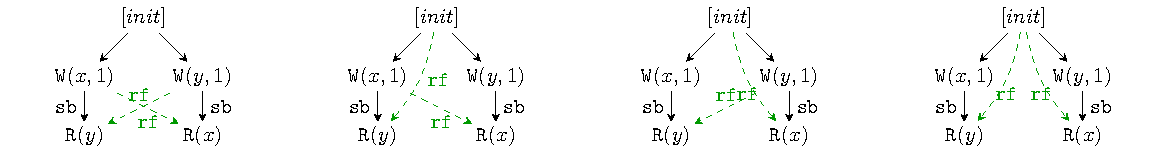
\includegraphics[scale=0.8]{figure/exec-graph/SB4.pdf}   
    \caption{Valid execution graphs of SB}  
    \label{SB4}  
\end{figure}



Lastly, the probability of encountering different executions is not uniformly distributed. Some execution graphs are more likely to be found, while others may have a lower probability of being discovered. Consider the example shown in Listing~\ref{P2}, where two threads update their corresponding flags \texttt{x1} and \texttt{x2}, and a third thread reads them. Suppose the test generator makes random decisions uniformly when adding events. The program printing 'A' requires one of the following orders shown in Table~\ref{tab:order-prob}, with a total probability of $\frac{7}{18}$, while printing 'B' has a probability of $\frac{11}{18}$.



\begin{table}[h]
    \centering
    \renewcommand{\arraystretch}{1.5} % 调整行高
    \begin{tabular}{|p{0.3\linewidth}|p{0.3\linewidth}|}    
        \hline
        order & probability  \\ \hline
        \texttt{w1} $\rightarrow$ \texttt{w2} $\rightarrow$ \texttt{r1} $\rightarrow$ \texttt{r2}  & $\frac{1}{3} \times \frac{1}{2} = \frac{1}{6}$ \\  
        \texttt{w2} $\rightarrow$ \texttt{w1} $\rightarrow$ \texttt{r1} $\rightarrow$ \texttt{r2} & $\frac{1}{3} \times \frac{1}{2} = \frac{1}{6}$ \\  
        \texttt{w1} $\rightarrow$ \texttt{r1} $\rightarrow$ \texttt{w2} $\rightarrow$ \texttt{r2} & $\frac{1}{3} \times \frac{1}{3} \times \frac{1}{2} = \frac{1}{18}$    \\ 
        \hline
    \end{tabular}
    \caption{Probabilities of each order}
    \label{tab:order-prob}
\end{table}

\begin{lstlisting}[caption={P2}, label={P2}]
atomic<int> x1 = {};
atomic<int> x2 = {};

void thread1() {
    x1 = 1;     // w1 
}
void thread2() {
    x2 = 1;     // w2
}

void thread3() {
    if(x1 == 1 /* r1 */ && x2 == 1 /* r2 */) {    
        print("A");
        assert(false);
    }
    else {
        print("B");        
    }
}
\end{lstlisting}



The process of the random walk test generation procedure is similar to the Galton board experiment. Consider the following $n$ level decision tree, from top to bottom, each step has two choices, either going left or right. Each node represents a state and the edges represent the decisions. There are some states that can be reached from multiple paths. Take the middle state in the second level for example, it can be reached by first choosing left then right, or by first choosing right then left. There are also some other states that have more strict requirements on the decision making. For example, the state circled in red requires always select the left choices to reach, with the probability of $\frac{1}{2^n}$. 
\begin{figure}[htbp]  
    \centering
    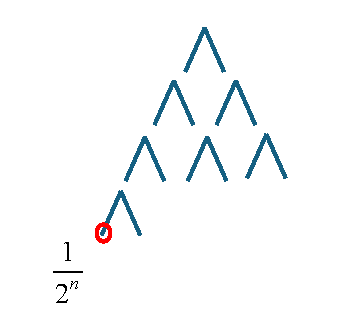
\includegraphics[scale=0.5]{figure/tree.pdf}   
    \caption{Random decision tree}  
    \label{tree}  
\end{figure}



If each time we start from the top and randomly make decisions, those states in the middle will be reached more frequently than those in the corners. However, if we can start from some middle states, it would be easier to reach some corner states, and hence the states reached in the end will be more diverse. This is where our fuzzer come to help. An intuitive description of the fuzzer is: whenever the fuzzer reaches a new state (i.e. finds an interesting execution graph), it mutates one of the decisions made. For the next iteration, the fuzzer replays the decision making until the mutated point, change the decision as mutated, and continues randomly afterwards. As shown in Figure~\ref{tree3} (a), suppose the red path is the previous exploration and the fuzzer mutates the second decision from going right to left (b). Then for the next exploration, it replays until the mutated choice and the probability of reaching the left corner state becomes $\frac{1}{2^{n-2}}$ (c). 

\begin{figure}[h!tbp]  
    \centering
    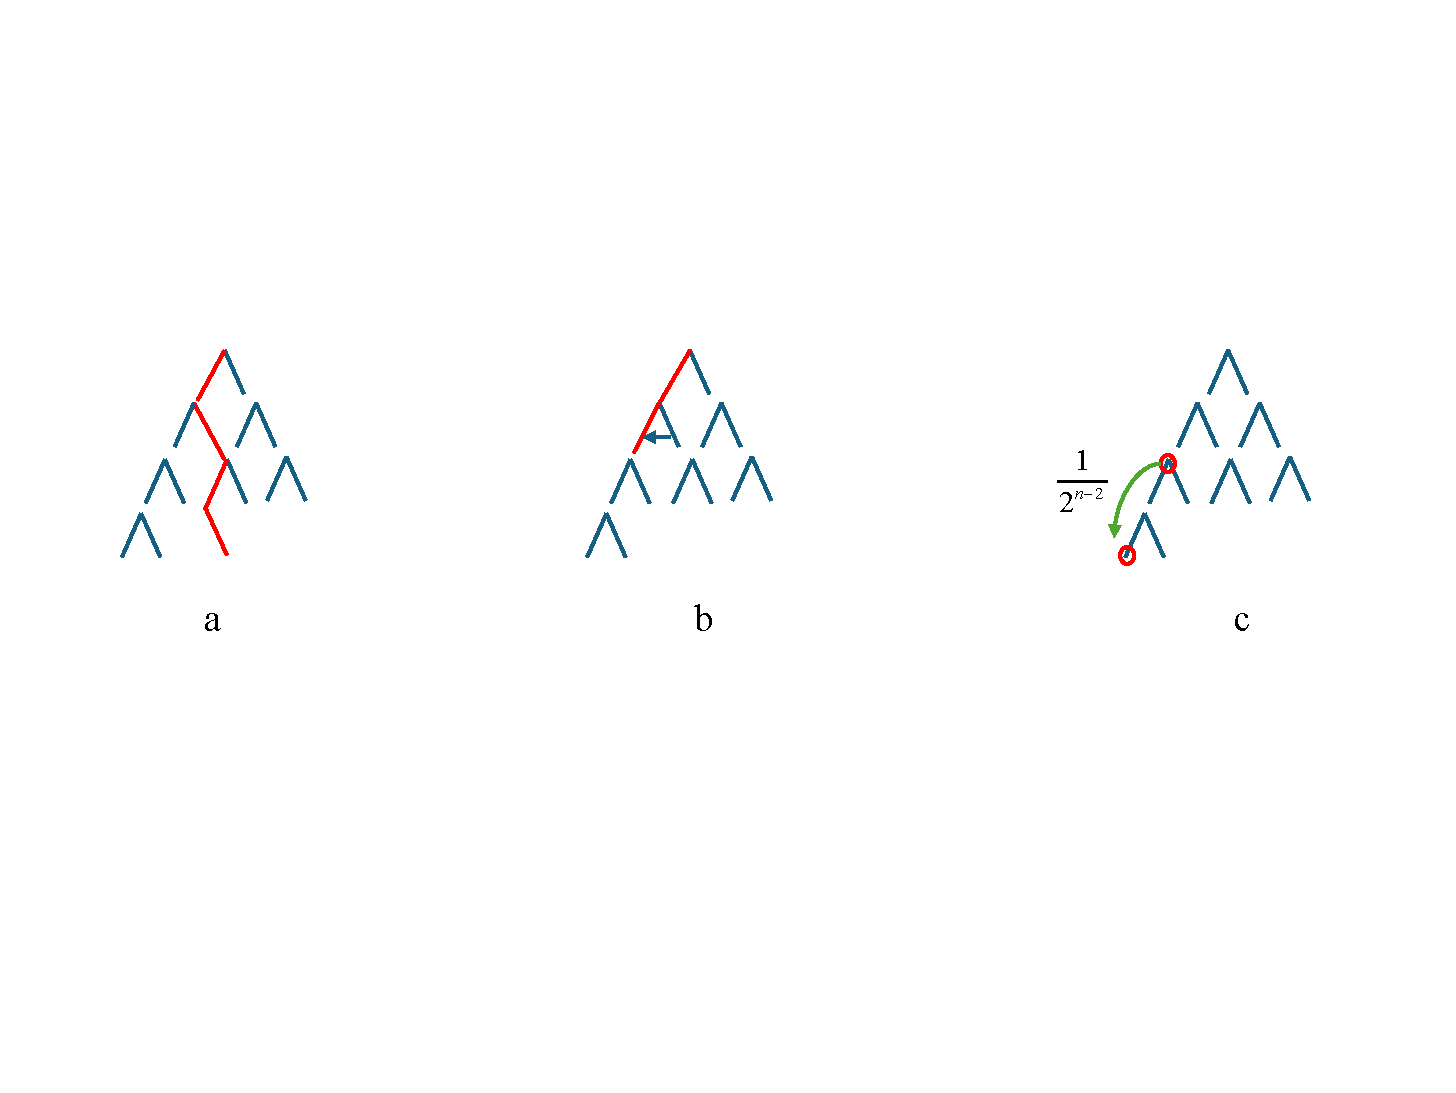
\includegraphics[scale=0.5]{figure/tree3.pdf}   
    \caption{Mutation}  
    \label{tree3}  
\end{figure}

% \michalis{Maybe the example above requires some more explanation. Assuming that a node in your tree is not an execution graph (but rather the rf choices within a graph), can it be the case that two paths yield the same graph? If so, why? If not, why does fuzzing help?}

Relating this to the randomized testing procedure, each parent node in the decision tree represents an intermediate state in the process of constructing a graph, while the leaf nodes represent completed graphs. The edges correspond to the scheduling or rf decisions made during exploration. Each time, the random walk tester restarts from the begining (top of the tree) and randomly generates execution graphs independently. However, due to the previously listed challenges, it often tends to generate a subset of frequently occurring execution graphs, sometimes repeatedly, leaving hard-to-find executions unexplored. We consider this approach inefficient and utilize fuzzing techniques to improve this. Ideally, the fuzzer should explore graphs with a more uniform frequency and broader coverage compared to  the random walk tester, as shown in Figure~\ref{tree-freq}.

\begin{figure}[h!tbp] 
    \centering
    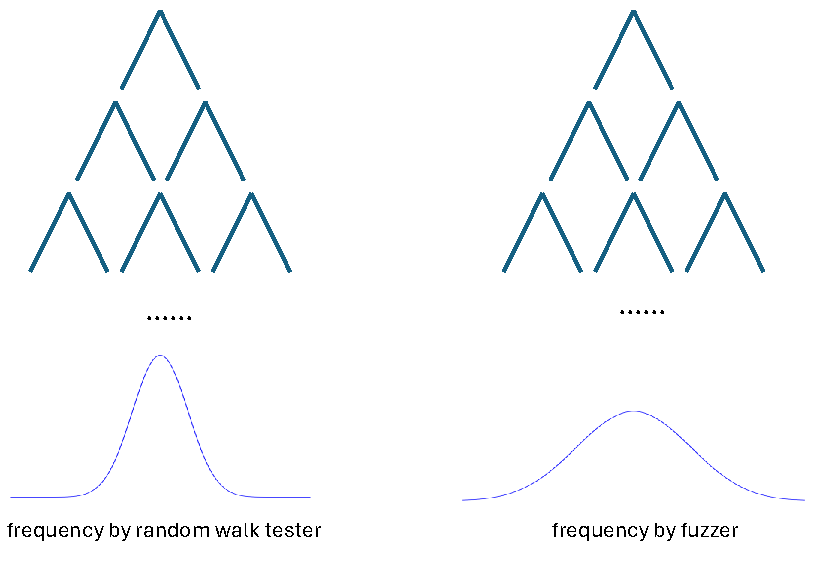
\includegraphics[scale=0.28]{figure/tree_freq.pdf} 
    \caption{Improvement of fuzzing}  
    \label{tree-freq}  
\end{figure}


The fuzzer aims to improve the performance of randomized testing approaches. Some random testers, such as C11Tester or GenMC in its estimation mode, use random walk testing. In contrast, exhaustive model checkers like GenMC explore all possible executions. Exhaustive checkers are useful when the search space is limited, typically when the program under test is not too large. Randomized testers are usually employed for testing larger programs. However, the drawback of this approach is that it does not retain state information between explorations, leading to redundant efforts. In our fuzzing algorithm, we track the explored execution graphs and mutate infrequent ones to guide the tester in covering a larger fraction of the graph search space.

\section{Example}

In this section, we present an example of the fuzzing approach on the execution graphs, using the \ref{exp-fuzz} program with release-acquire pairs. 

\begin{lstlisting}[caption={Fuzzing example}, label={exp-fuzz}]
    atomic<int> x = {};
    
    void thread1() {
        x.store(1, release);    // w1
        x.store(2, release);    // w2
    }
    void thread2() {
        auto r1 = x.load(acquire);    // r1
        auto r2 = x.load(acquire);    // r2
    }
    \end{lstlisting}



Suppose during exploration, one execution graph is constructed as shown in Figure \ref{example_construct}, where the labels of events and relations are omitted. The read values in \texttt{thread2} are both 2. In this execution, \texttt{r2} has only choice to read from, which is \texttt{w2}, since \texttt{r1} has already read from \texttt{w2} and \texttt{r2} reading from w1 will introduce a cycle in the graph. However, \texttt{r1} can have two choices: \texttt{w1} and \texttt{w2}. If the fuzzer consider this execution as interesting and change the rf choice for \texttt{r1}, a new execution can be revealed in the next iteration, as shown in Figure \ref{example_mutate}. 

\begin{figure}[htbp] 
    \centering
    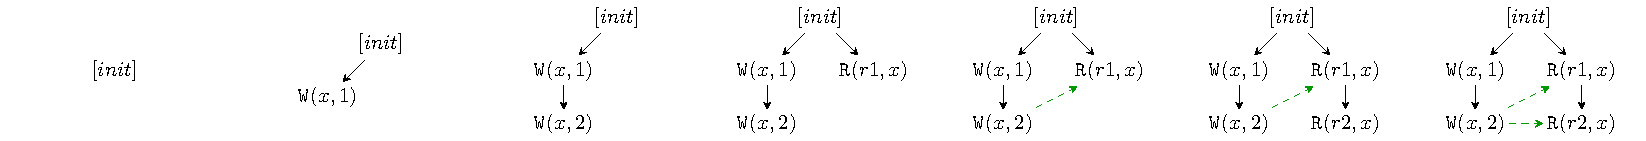
\includegraphics[scale=0.52]{figure/exec-graph/example_construct.pdf} 
    \caption{Construction of an execution graph} 
    \label{example_construct} 
\end{figure}

\begin{figure}[htbp] 
    \centering
    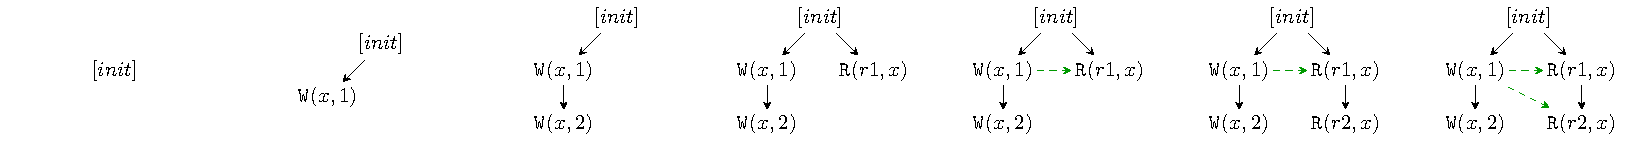
\includegraphics[scale=0.52]{figure/exec-graph//example_mutate.pdf} 
    \caption{Mutate the previous execution graph and re-explore} 
    \label{example_mutate} 
\end{figure}

% \michalis{Why can't you get r1 = 1 with testing? A different motivation is required.}
%\burcu{Could you provide an example of the fuzzing approach on the execution graphs? E.g., Give an example program and a random execution graph of the program. Then, show another execution graph that is obtained by some mutation (e.g., mutates the prev. graph after some prefix) and exposes another behavior of the program.}

\section{Overview}


This section provides a high-level overview of the fuzzing algorithm. The implementation details and evaluation results will be presented in later chapters.


The fuzzer uses partially constructed graphs, represented by "prefixes" in the following context, as guidance for further explorations. As shown in Algorithm~\ref{fuzzer}, the fuzzer executes the program $P$ a total of $N$ times (line~\ref{line:input}), generating an execution graph each time after exploring the search space. It maintains a set of prefixes, initially empty (line~\ref{line:init_prefix}). At the beginning of each exploration, it picks a prefix from the prefix set (line~\ref{line:pick_prefix}). If no prefixes are available in the set, the exploration will be entirely random (line~\ref{line:random_explore}). With a selected prefix, the fuzzer replays the execution up to the end of the prefix and randomly constructs the remaining part of the execution graph (line~\ref{line:explore_prefix}). When the exploration is finished, an execution graph is constructed, and the fuzzer determines whether this graph is interesting according to certain metrics (line~\ref{line:is_interesting}). A graph is considered interesting if it is a new execution graph or contains new relations or events. The interesting graph is then mutated to generate new prefixes (line~\ref{line:mutate}). These new prefixes are added to the prefix set for future use (line~\ref{line:add_prefix}). For example, the fuzzer might modify a reads-from relation in the graph and remove the invalid portion following that relation to create a prefix. The fuzzer may also dynamically discard some prefixes based on their effectiveness in finding new interesting graphs. New graphs are added to the graph set (line~\ref{line:add_graph}) and are ultimately outputted at the end (line~\ref{line:output}). 


% \michalis{Why execute only up to N times? Could you do this with a time budget too? If so, mention this.}

\begin{algorithm}
    \caption{Fuzzing algorithm}
    \label{fuzzer}
    \begin{algorithmic}[1]
    \STATE \textbf{Input:} Program $P$ and number of explorations $N$ \label{line:input}
    \STATE \textbf{Output:} $N$ execution graphs
    
    \STATE prefix\_set $\leftarrow \emptyset$ \label{line:init_prefix}
    \STATE graphs $\leftarrow \emptyset$ 
    
    \FOR{$i \leftarrow 1$ \TO $N$}
        \IF{prefix\_set $\neq \emptyset$}   
            \STATE $p \leftarrow$ get\_prefix(prefix\_set) \label{line:pick_prefix}
            \STATE $g \leftarrow $ explore\_from\_prefix($p$) \label{line:explore_prefix}
        \ELSE 
            \STATE $g \leftarrow $ explore\_randomly() \label{line:random_explore}
        \ENDIF 
        \IF{is\_interesting(g)} \label{line:is_interesting}
            \STATE $p' \leftarrow$ mutate(g) \label{line:mutate}
            \STATE prefix\_set $\leftarrow$ prefix\_set $\cup p'$      \label{line:add_prefix}  
        \ENDIF
        \STATE graphs $\leftarrow$ $graphs \cup g$      \label{line:add_graph}
    \ENDFOR
    
    \RETURN graphs      \label{line:output}
    \end{algorithmic}
\end{algorithm}

The following are a few notes regarding this algorithm.

\paragraph*{$N$ as an input parameter} The number of unique execution graphs in the outputted graph set is a major metric for evaluating the fuzzer's searching ability. The algorithm takes a fixed number of iterations, $N$, as an input parameter. This facilitates the comparison of algorithmic efficiencies regardless of implementation details. In practice, execution time is also an important consideration. In our fuzzer implemented with GenMC, described in Chapter~\ref{cha:genmc}, we also evaluate the fuzzer by running it for a fixed time budget and count the number of unique executions found.

% hash 
\paragraph*{Counting the number of unique graphs} In order to count the number of execution graphs, we will also need a hash function that maps the set of graphs, $G$, to a subset of integers, $H$. This hash function, $h: G \to H$ should be a bijection. That is, it should satisfy the following properties:
\begin{itemize}
    \item $h$ is surjective: The same execution graphs should always have the same hash values. This requires the hash function to exclude irrelevant information, such as the timestamps of events, which is related to specific explorations. 
	\item $h$ is injective: Different execution graphs should have different hash values. This requires the hash function to include enough information from the graphs, such as the rf relations. Ideally, there should be no hash collisions, but as this is a low-probability event, it can be ignored within the scope of our work.
\end{itemize}

If $h$ is bijective, the size of the set of hashes, $|H|$, equals that of execution graphs (i.e. they are equinumerous), and can thus be used to count the number of distinct graphs. In our implementations, we use different hash functions due to the differing internals of the C11Tester and GenMC, but both are considered bijective functions.

% \paragraph*{The is\_interesting function} This function operates on execution graphs as a feedback metric in the fuzzing loop. Conceptually, it serves as a connecting point of the beginning and end of an exploration procedure. Telling whether an execution graph is interesting helps the fuzzer to decide whether to mutate it and can also indicate the ability of finding interesting graphs of the mutated prefixes. If a prefix can find more interesting graphs, it should be prioritized in use. 

\paragraph*{The is\_interesting Function} 
This function evaluates execution graphs as a feedback metric in the fuzzing loop. Conceptually, it serves as a connecting point between the beginning and end of the exploration procedure in two folds:
\begin{itemize}
    \item Backwards: It assesses the performance of mutated prefixes based on their ability to find interesting graphs. Prefixes that lead to more interesting graphs should be prioritized for use.
    \item Forwards: It determines whether an execution graph is interesting, which helps the fuzzer decide whether to mutate it. An interesting execution graph indicates the potential for discovering other interesting graphs through mutation.
\end{itemize}

 




In the following chapters, we present two fuzzers based on C11Tester and GenMC, both of which implement the fuzzing algorithm, with different implementations for functions such as is\_interesting, mutate,  explore\_from\_prefix and the hash function.


% \michalis{Why does it matter whether g is interesting? Isn't it more important that the mutated graph is interesting?}






% \subsection{Threads}





 
\chapter{\label{cha:c11tester}Fuzzing with C11Tester}

C11Tester is a automatic testing tool that supports a large gragment of C/C++ weak memory model. This chapter presents an overview of C11Tester and customazation points of its plugable framework. Then the fuzzer's implementation is described. Finally we show the evaluation results on some of the benchmarks.

\section{Overview of C11Tester}

The C11Tester contains the following basic constructs: insstrumentation, scheduler, consistency checker and race detecter.

C11Tester uses a LLVM pass compiler pass, CDSPass, to instrument all atomic operations, non-atomic accesses to shared memory locations, thread functions, mutex operations and fence operations by inserting a corresponding function call. The compiled program is linked with a dynamic library containing the function calls.
C11Tester impelments a thread library that supports the same APIs of C++'s standard library and Posix thread library. The user's thread function calls will be mapped into user space fibers, instead of kernel space threads. Thus, all threads will be executed in a sequential manner with scheduling managed by a central scheduler, which is provided by the C11Tester. A context switching approach is applied to simulate the interleavings of threads to improve efficiency.
Each atomic operation, thread creation and joining, mutex locks and unlocks, and memory fences will create a Action object, containing its type, value, memory order, thread id and other runtime information. Since all threads are sequenced during execution, each action will have a unique sequence number. The relations between actions, such as read from and synchronized with, are also maintained by the Action class.

Although C/C++ programs under weak memory model do not use scheduling semantics, C11Tester does contain a central scheduler. It's worth noting that the scheduler do not simulate schedulings of threads, instead, it's designed to check actions of different threads in a total order. This is based on the implementation of mapping user's threads into fibers and checking them sequentially. All actions within the same thread will be checked following their sequence order, as a step, and the scheduler decides whether to check actions of other threads in the next step. Hence, two decisions will be made in each step, the behavior of the current action and the next thread to select. If the current action is a read, C11Tester will choose a write action to read from. Since the read-modify-write operations are instrumented with two functions, a read and a write, the scheduler ensures these two actions are atomic, i.e. to check them without switching to other threads in between.

Memory locations are devided into two types: atomic locations and non-atomic locatios. Non-atomic access to shared memory locations is the source of introducing data races. C11Tester implements a race detecter to check data races. The race detecter will allocate a chunk of shadow memory for each of the non-atomic memory locations. Loading from or writing to non-atomic shared variables are instrumented with specific functions, which will register the current thread's state to the shadow memory. When multiple concurrent access to some shared non-atomic memory with at least one of them being a write is detected, a data race will be reported.

Here we use an example to demonstrate the process of C11Tester's model checking procedure.

\begin{lstlisting}[caption={P3}, label={P3}]
#include "librace.h"
#include <atomic>
#include <thread>
uint8_t data = {};
std::atomic<int> flag = { 1 };  

// thread 2
void t2() {
    store_8(&data, 0);          // cds_store8    
    flag.store(1, mo_release); 
}

// thread 3
void t3() {
    if (flag.load(mo_acquire))
        store_8(&data, 1);
}

// thread 1
int main() {
    std::thread thrd2(t2);
    std::thread thrd3(t3);
    thrd2.join();
    thrd3.join();
}
\end{lstlisting}

In this program, there are two shared variables: non-atomic variable data and atomic flag. The librace.h header is provided by C11Tester, containing the instrumented function store\_8 for non-atomic variables. The initialization of flag, which is non-atomic, deliberately uses 1 as the initial value. Since the c++ standard thread library internally calls POSIX APIs, the thread-related function calls will be hooked by C11Tester's dynamic library.

After compilation, the model checker launches the program. After initializing the global variables, the model checker creates the first thread, which is the main thread and assign an tid, 1, to it. The first event is creating thrd2. After thrd2 is created and assigned an tid of 2, two threads, main and thrd2, are active. The model checker will randomly pick a thread to continue. Suppose the main thread is selected, the next event of it is creating thrd3. After creating thrd3, the next event of main is joining thrd2, so it becomes inactive. Now the current active threads are: thrd2 and thrd3.

If the model checker selects thrd2, the two events in it, writing to data and flag, will be consumed, and the thrd2 is finished. Now thrd2 becomes joinable and the currently active threads are: main and thrd3. Suppose main is selected and after joining thrd2 it becomes inactive again. Then thrd3 becomes the only active thread so it will be executed without the need to make a choice. The first event in thrd3 is loading the value of flag. Since the store of flag in thrd2 has already been explored, the non-atomic initialization of flag is hidden in the modification order. Hence only the atomic store is visible to this load, and the rf relation also forms a synchronization-with relation between the two thread. When writing to the non-atomic data, the race detecter checks pervious access to that location. The store in thrd2 happens before the read in the current thread, which happens before the current store, so all events are totally ordered and no data race will be reported.

Considering another case, suppose the model checker selects thrd3 after creating both threads. The load of flag will be executed and only the initialization of data is visible to it. After reading the initial value, the store of data is consumed. When thrd3 is finished, the stores in thrd2 will be executed. When writing to data, the race detecter checks previous actions relating to that memory location. The store in thrd3 is already explored and it has no happen before relations with the current store, so the two stores are concurrent and a data race is reported.

One optimization that C11Tester implements is that it will consume writes with release and relaxed memory orders, only pausing on sc writes. This is because the sc order is part of the C/C++11 memory model so different sc order will result in different executions. Besides, consuming the weak writes will not lose the ability to cover possible executions. Consider the following example  \ref{P4},
\begin{lstlisting}[caption={P4}, label={P4}]
    std::atomic<int> var = {};      // (w0)
    void t2() {
        auto _ = var.load(acquire); // (r1)
    }
    void t3() {
        var.store(1, sc);           // (w1)
        var.store(2, release);      // (w2)
        var.store(3, release);      // (w3)
    }
\end{lstlisting}
after creating two threads, if t2 is selected first, r1 can only read from the initial value. If t3 is selected, the first event, w1, in this thread will be executed. The next two events are release writes, so the model checker will not re-select threads after w1. Instead, it will execute w2 and w3 until t3 is finished. Then it finds the only active thread is t2, so it selects t2. Now the set of available writes for r1 to read from becomes: w1, w2 and w3, and r1 is free to randomly select one of them. Although making thread decisions after each event is also feasible, the optimized version is more efficient and still able to cover all 4 possible executions.

Another optimization performed by C11Tester is that it avoids backtracking during exploration. To achieve this, it performs consistency checking at each step to ensure it's valid. It make decisions based on the implications of the memory model and already explored events. In \ref{P4} for example, if t3 has been explored, when choosing the rf relation for r1 in t2, the rf-set only contains w1, w2 and w3, where w0 is excluded. If r1 had selected w0 and the model checker continues until some point where the execution graph is found to be infeasible under the memory model, it would have to perform backtracking to make a different choise for r1. Consider another example \ref{P5},
\begin{lstlisting}[caption={P5}, label={P5}]
    std::atomic<int> var = {};      // (w0)
    void t2() {
        auto _1 = var.load(acquire); // (r1)
        auto _2 = var.load(acquire); // (r2)
    }
    void t3() {
        var.store(1, sc);           // (w1)
        var.store(2, release);      // (w2)
        var.store(3, release);      // (w3)
    }
\end{lstlisting}
if r1 has already seelcted w3 to read from, only w3 will be included in the rf-set for r2, becuase w3 $\xrightarrow{\text{rf}}$ r2 implies that w0-2 are modification-ordered before w3 and thus should not be visible to r2, which is sequence ordered after r1. Otherwise the RR coherence will be violated. Excluding infeasible writes from the rf-set ensures the rf's to be valid, which in turn avoids the backtracking efforts.

To summarize, C11Tester will execute the program from beginning to end, randomly picking threads and writes, with the optimizations of consuming weak writes and constraining rf-sets.


\section{Customazation points of C11Tester}

C11Tester provides two interfaces: selectWrite and selectThread that randomly selects a thread or write from a provided set. These two functions can be overwritten to implement new fuzzers. The provided set already excludes invalid choices so it's safe to pick other choices in the set. Thus we can define two types of mutations: changing the next thread to be added or changing the write that a read event reads from.

\section{Fuzzer implementation}

To implement a fuzzer described in Algorithm \ref{fuzzer}, there are several specific functions to be defined:

\begin{itemize}
	\item A hash function that computes a unique identifier for an execution graph, which is used to indicate whether the execution graph has been encountered before and to count the number of unique executions that are found in the end of N iterations.
	\item A function that returns a boolen that indicates whether the execution graph is interesting.
	\item A function that mutate the previous execution graph and produces a prefix of the mutated graph.
	\item A function that enforces the prefix, i.e. replays until the mutated choice.
\end{itemize}

The hash function for executioin graph encodes: event types, memory orders, reads-from relations. It first iterate threads by their thread ids, and for each event in each thread, it computes the hash of its event type and memory order (for atomic operations). If the event is a read event, it also combines the hash of the write event it reads from. To be noticed, in this hash function the modification order is not included although it's part of the execution graph under many memory models. This is because the hash function only cares about observable behaviours, such as read values, which may be influenced by modification orders. However, changing some modification orders may or may not change the observable behaviours. The hash function is defined in Algorithm \ref{c11fuzzer-hash} as follows:


\begin{algorithm}
	\caption{Hash of execution graphs}
	\label{c11fuzzer-hash}
	\begin{algorithmic}
		\STATE \textbf{Input:} Execution graph $g$
		\STATE \textbf{Output:} Hash value $h$

		\STATE h $\leftarrow$ 0
		\FOR{each $i$ from 0 to g.max\_tid()}
		\STATE events = g.get\_events\_in\_thread(i)
		\FOR{each $e$ $\in$ events}
		\STATE h $\leftarrow$ hash\_combine(h, e.type)
		\STATE h $\leftarrow$ hash\_combine(h, e.memory\_order)
		\IF{e is a read event}
		\STATE h $\leftarrow$ hash\_combine(h, e.rf)
		\ENDIF
		\ENDFOR
		\ENDFOR
		\RETURN $h$
	\end{algorithmic}
\end{algorithm}

The is\_interesting function returns true if the hash of the current execution graph is not covered in previous explorations. This is the least restrictful metric, alternatively, it can be defined as returning true if new rf relations has been covered. Another possible definition is to check whether the execution graph reveals a new bug, which is biased on searching for bugs. In our definition, we aims to find more new executions, with more new buggy executions being a by-product.

The mutate function uniformly picks a fixed number of decisions, including threads and rf's, with multiple choices in the provided set. For each of them, it mutates the selected decision and cuts out the rest decisions to produce a prefix. Since the only two places where randomness is used are selectWrite and selectThread, the choices of threads and writes will be uniquely mapped to an execution graph. Hence the prefix of a decision trace also defines a prefix of an execution graph.

% 画图

The mutated prefixes will be added to a prefix set. The replaying function choose a prefix from the set and enforce C11Tester to make the same decisions in that prefix. After enforcing the prefix,  C11Tester is switched to the random mode, continuing random exploration until the graph is completed.

\section{Benchmarks}

The fuzzer and C11Tester are tested under 11 benchmarks: barrier, chase-lev-deque, mpmc-queue, linuxrwlocks, mcs-lock, dekker, rwlock, seqlock, bipartite-buf, left-right and ring-buf. Some of them are collected from open source libraries, others come from the original C11Tester's benchmark set, which are also taken from open source libraries, internet discussions and papers. Here is a list of descriptions of these benchmarks:

\paragraph{barrier} It comes from a solution of StackOverflow discussion. It implements a spinning barrier that halts a fixed number of threads to wait and releases the barrier when all threads are waiting. It maintains a counter for the number of threads that are waiting so far and a step state that counts the number of barrier synchronizations. It was injected with a bug of using the relaxed memory order of the counter.

\paragraph{chase-lev-deque} An implementation of the Chase-Lev deque data structure using the C11 primitives. It was published in \cite{chase-lev-deque-impl} but found to have bug in its implementation, due to the use of relaxed operations of fences.

% TODO: ref
\paragraph{mpmc-queue} A multi-producer multi-consumer queue implementation from a blog post \cite{mpmc-queue-impl}.

\paragraph{linuxrwlocks} A reader-writer lock implementation from the Linux kernel. An rwlock only allows one writer at a time but can allow multiple readers to access the protected data.


\paragraph{mcs-lock} A list-based contention-free lock originally proposed by Mellor-Crummey and Scott\cite{mcs-lock}. The implementation comes from \cite{mcs-lock-impl}. In this data structure, each thread maintains a node of a queue. When a thread wants to lock, it asks the mutex to set its tail of the queue to be the thread's node. When other threads lock, they have to wait for the tail to be removed by the mutex.

\paragraph{dekker} A Dekker's critical section algorithm implemented with fences \cite{dekker-fence-impl}. This algorithm ensures only one thread can enter critical section at a time. A shared turn variable records which thread is taking the turn. Each thread has a flag variable to indicate its state. Before entering the critical section, a thread should first raise its own flag and then check whether the turn is not set. All atomic operations on the turn and flags are relaxed but fences are used to synchronize concurrent accesses.

\paragraph{rwlock} Another rwlock implementation similar to linuxrwlocks.
\paragraph{seqlock} A sequence lock implementation. The lock protects some shared data using an atomic counter, initialized 0. A writer increments the counter twice, both in the beginning and end of writing. Hence whenever the counter is odd, there must be some other thread modifying the data, so other threads have to wait.

\paragraph{bipartite-buf} A single-producer-single-consumer test for a bipartite buffer implementation written in C++11, customazed from \cite{lockfree-DNedic}. The bipartite buffer is a variation of the ring buffer which allows in-place processing with linear space guarantee.

\paragraph{left-right} A generic implementation \cite{lockfree-xenium} of the LiftRight algorithm\cite{left-right}. The algorithm functions similarly to the reader-writer lock, but ensures non-blocking for reads. It uses two instances for the protected data, one of which is used for all reader threads. The writer thread will work on the other instance and after writing is finished, two instances are switched.


\paragraph{ring-buf} A ring buffer that supports adding or removing multiple objects simultaneously \cite{lockfree-DNedic}. It maintains two indexes, a read and a write index of the buffer. After adding or removing, these two indexes will be updated to appropriate values.


\burcu{TODO: Briefly describe each benchmark}

\section{Evaluation and discussion}

\burcu{TODO: List the research questions you explore, and answer the questions using your experimental results.}
\burcu{Do you have some results for the larger benchmarks in C11Tester?}



\paragraph*{Research questions} The following research questions are list for evaluating the fuzzing algorithm.
\begin{enumerate}[label=RQ\arabic*]
	\item Does the fuzzer detects the bug ealier than the random tester? \label{RQ:hardbug}
	\item Is the fuzzer able to cover a larger range of execution graphs comparing to other random-based exploration strategies? \label{RQ:coverage}
	\item When the program has bugs, will being able to detect more bugs come as a byproduct of covering more execution graphs \label{RQ:bug}
	\item How does the fuzzer cause overhead in C11Tester in real-world applications? \label{RQ:overhead}
\end{enumerate}

To address the research questions, we use the benchmarks to test our fuzzer and other approaches with same amout of iterations, $N$, and compare their results. If not specifically stated, $N = 10000$.

\subsection{\ref*{RQ:hardbug}: Fuzzer vs C11Tester}

One important metric for a fuzzer is whether it's able to detect the bug effectively. In this section, we use several programs with some hard-to-find bugs and examine the iterations taken to find a bug for the fist time, denoted as $N_{bug1}$. The smaller $N_{bug1}$ is, the more effective the fuzzer or the tester is. Table \ref{c11fuzzer-hardbug} shows $N_{bug1}$ of the fuzzer and the random tester, where dash means not able to detect the bug.

\begin{table}[h!]
	\centering
	\begin{tabular}{ |c|ccccc| }
		\hline
		Benchmarks & bipartite-hard & long-race & mp & P1  & reorder\_10 \\
		\hline
		C11Tester  & 1170           & -         & 2335  & 489 & 9           \\
		C11Fuzzer  & 754            & 717       & 30 & 74  & 9           \\
		\hline
	\end{tabular}
	\caption{Iterations taken to detect the first bug}
	\label{c11fuzzer-hardbug}
\end{table}


Take the long-race benchmark for example. This benchmark is taken from the rff's repository, customazed with relaxed memory operations, as shown in Listing. \ref{long-race}.

\begin{lstlisting}[caption={long-race}, label={long-race}]
	std::atomic<size_t> sum{ 0 };
	std::atomic<size_t> dif{ 0 };
	
	// thread 2
	void* sub_worker(void* arg) {
		if (sum.load(relaxed) == 1) {
			dif.fetch_sub(1, relaxed);
			if (sum.load(relaxed) == 2) {
				dif.fetch_sub(1, relaxed);
				if (sum.load(relaxed) == 3) {
					dif.fetch_sub(1, relaxed);
					if (sum.load(relaxed) == 4) {
						dif.fetch_sub(1, relaxed);
					}
				}
			}
		}
		return NULL;
	}
	
	// thread 3
	void* add_worker(void* arg)	{
		sum++;
		if (dif.load(relaxed) == -1) {
			sum.fetch_add(1, relaxed);
			if (dif.load(relaxed) == -2) {
				sum.fetch_add(1, relaxed);
				if (dif.load(relaxed) == -3) {
					sum.fetch_add(1, relaxed);
					if (dif.load(relaxed) == -4) {
						fprintf(stderr, "Bug found\n");
						abort();
					}
				}
			}
		}
		return NULL;
	}
\end{lstlisting}

Hitting the bug requires two workers to modify the shared variable alternately, in a very strict order (we also tested the long-race benchmark with rff, and it took 15 thousand iterations to detect it). There are in total 9 different executions of this program. Figure.\ref{graph-freq} shows how many times each execution graph (represented by their hashes in x-axis) are explored in $N$ iterations. It can be observed that the random tester is mostly biased on the first and second executions, which together take up 96.5\% of $N$. On the contrary, the fuzzer exhibits a more "flattened" frequency plot on executions and covers all 9 execution graphs. This is caused by the mutations on those infrequent executions during exploration. 

Figure.\ref{hardbug:bipartite-buf-hard} to \ref{hard:reorder-10} show the number of unique executions and bugs found in first 1000 iterations. It can be observed that the fuzzer detects the bug ealier than C11Tester and also covers a higher range of executions.

\begin{figure}[htbp] 
    \centering
    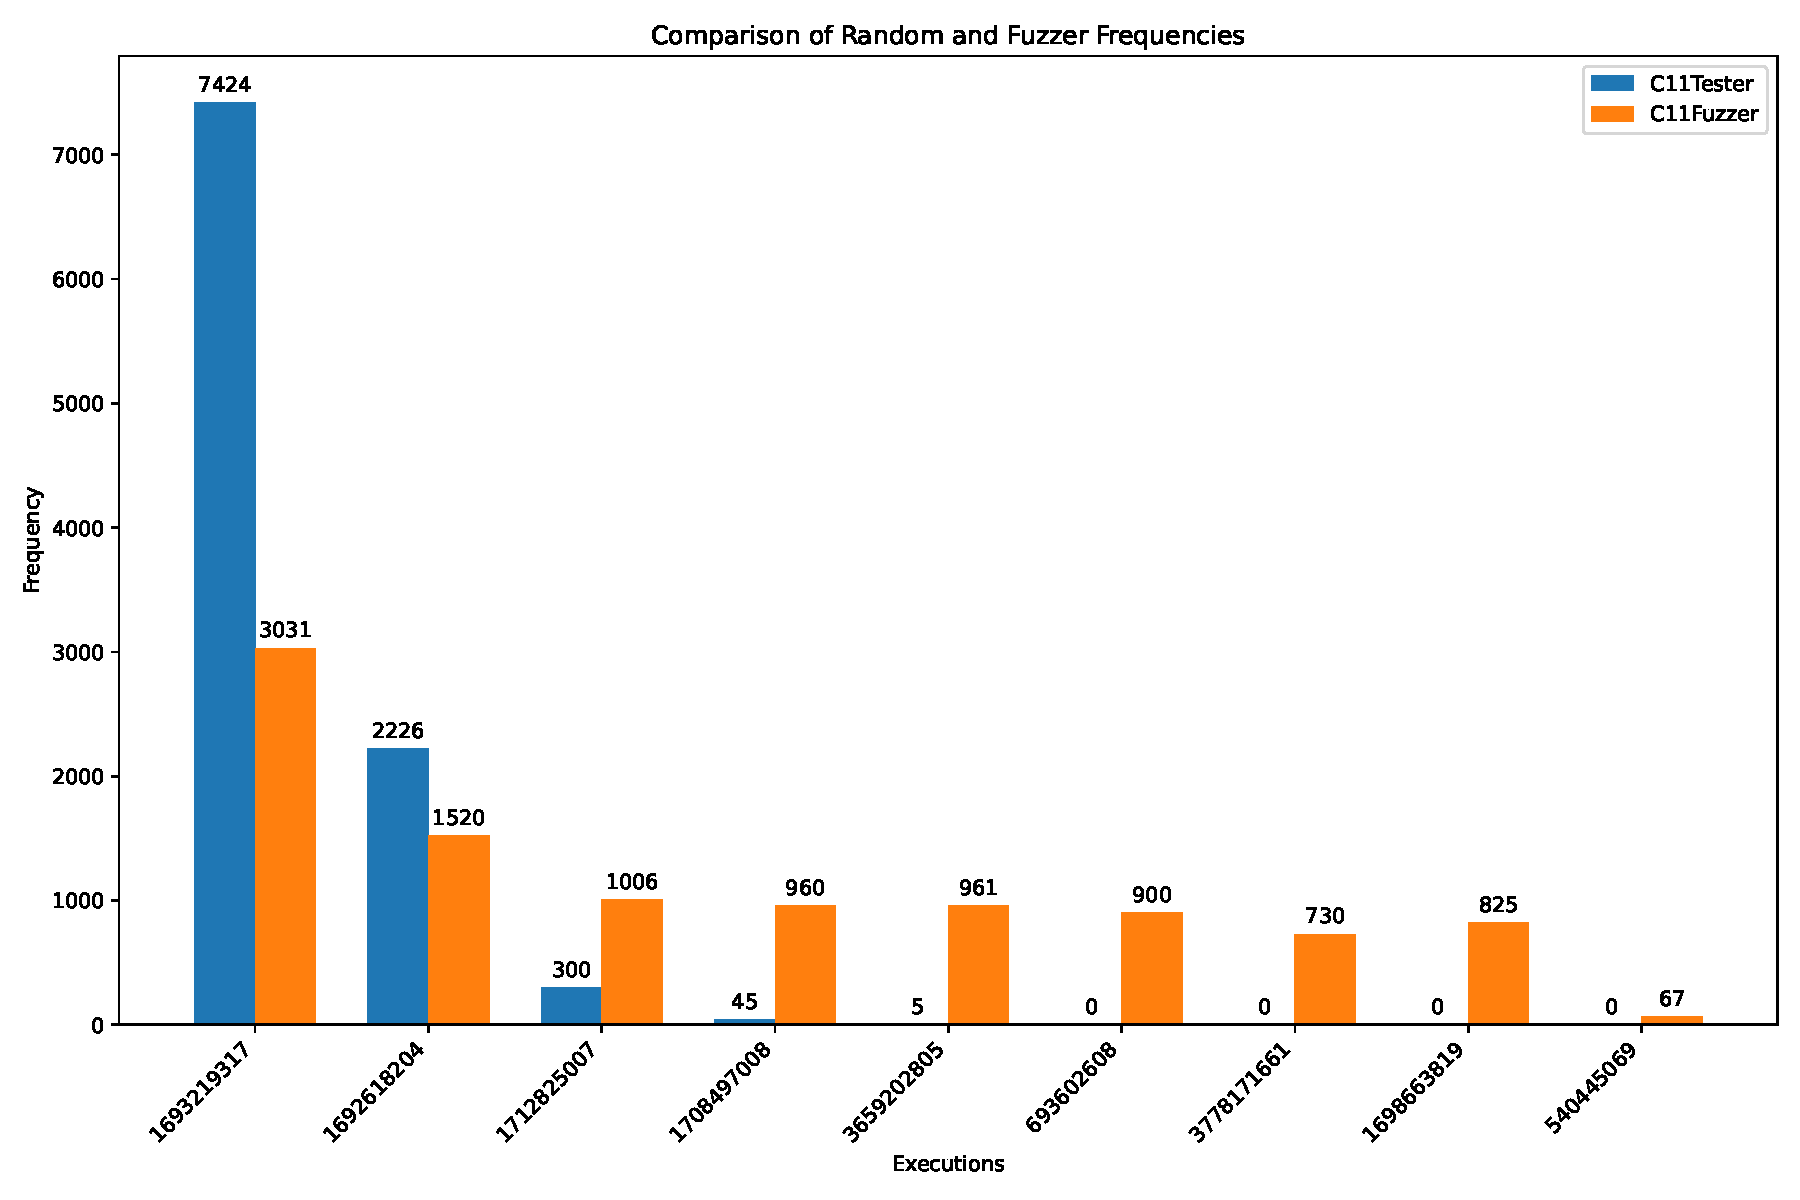
\includegraphics[scale=0.35]{figure/hardbug/long-race_freq.pdf}  
    \caption{Frequencies of execution graphs } 
    \label{graph-freq} % 图片标签,用于交叉引用
\end{figure}


\begin{figure}[H]

	\centering
	\begin{minipage}{0.45\textwidth}
		\centering
		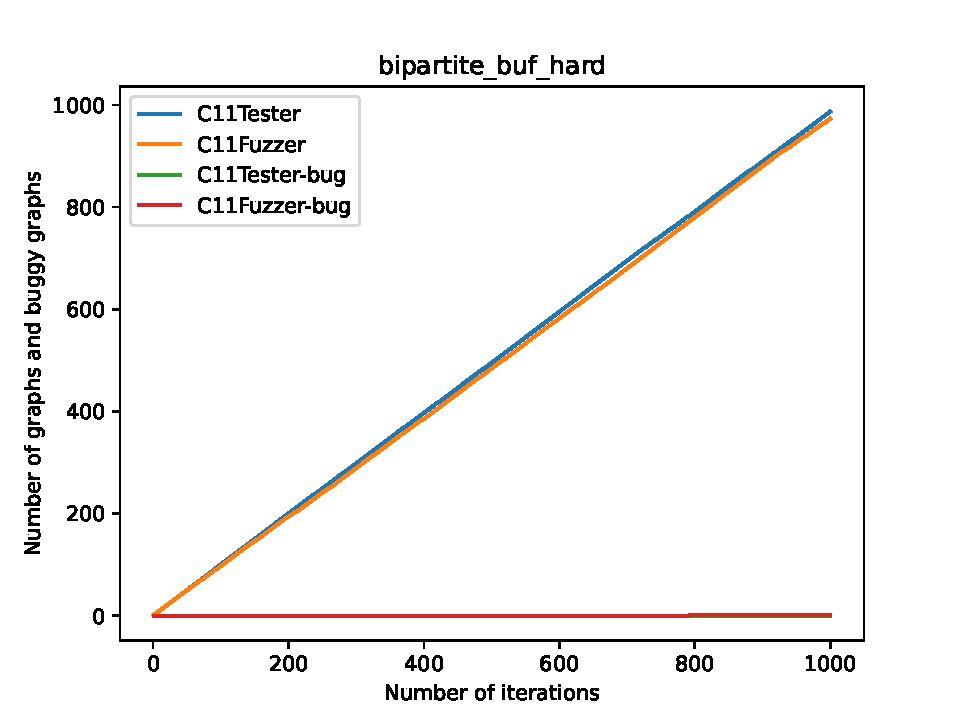
\includegraphics[width=\textwidth]{figure/hardbug/bipartite_buf_hard_bug.pdf}
		\caption{bipartite-buf-hard}
		\label{hardbug:bipartite-buf-hard}
	\end{minipage}
	\hfill
	\begin{minipage}{0.45\textwidth}
		\centering
		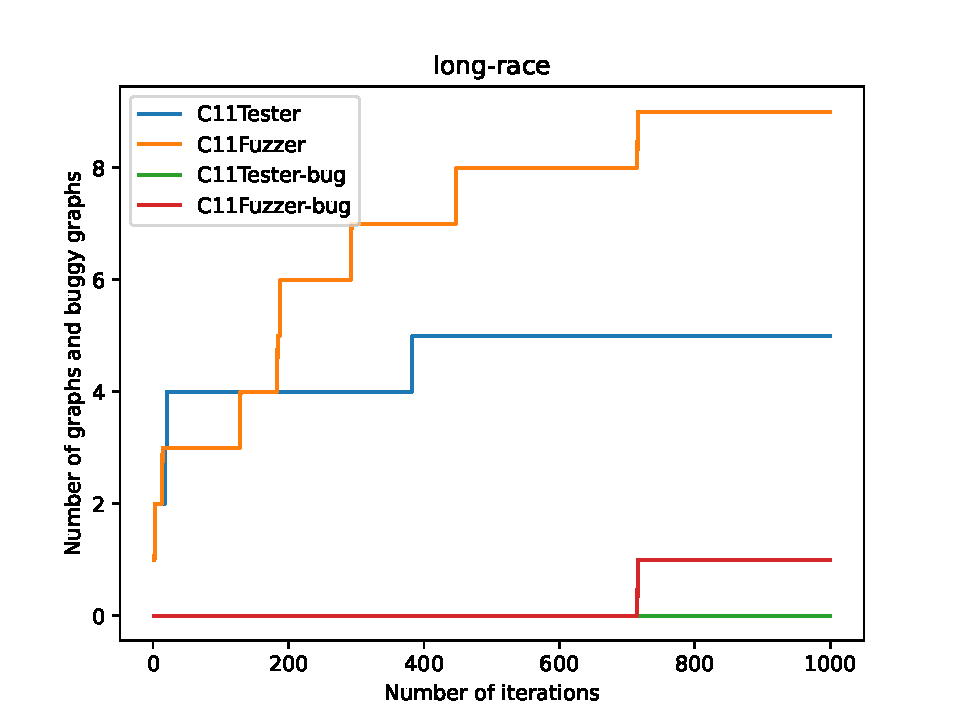
\includegraphics[width=\textwidth]{figure/hardbug/long-race_bug.pdf}
		\caption{long-race}
		\label{hardbug:long-race}
	\end{minipage}

	\vspace{0.5cm}

	\begin{minipage}{0.45\textwidth}
		\centering
		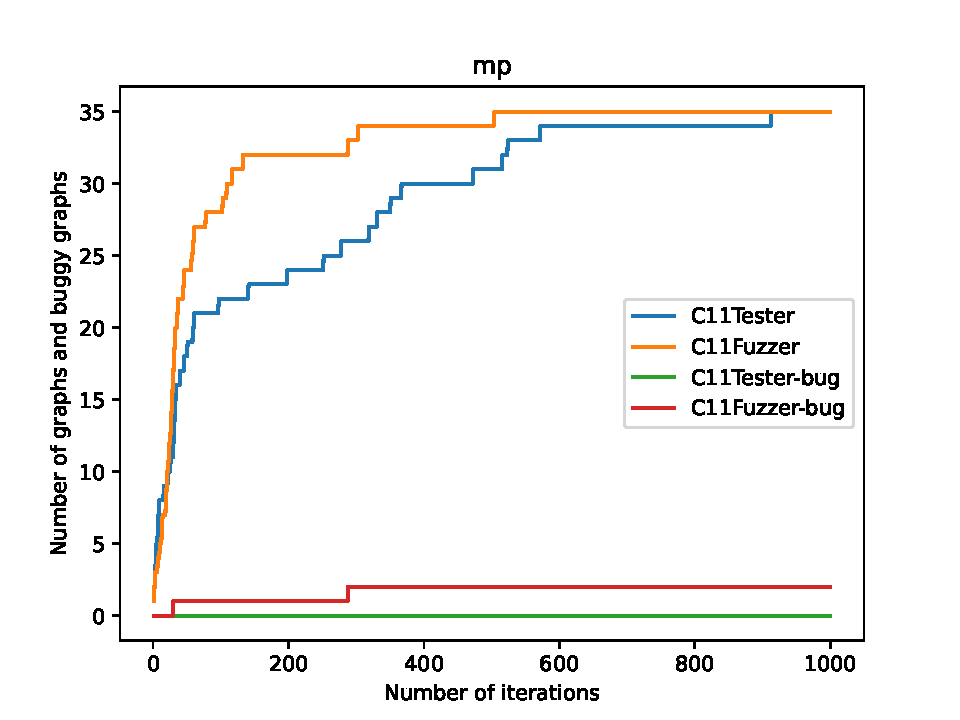
\includegraphics[width=\textwidth]{figure/hardbug/mp_bug.pdf}
		\caption{mp}
		\label{hardbug:mp}
	\end{minipage}
	\hfill
	\begin{minipage}{0.45\textwidth}
		\centering
		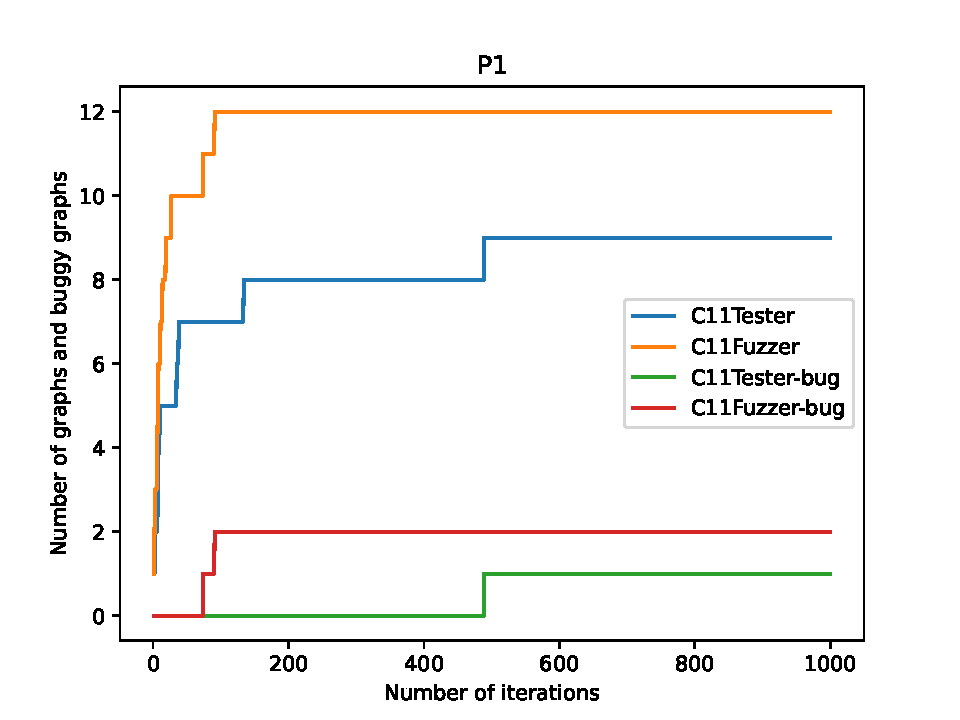
\includegraphics[width=\textwidth]{figure/hardbug/P1_bug.pdf}
		\caption{P1}
		\label{header:P1}
	\end{minipage}

	\vspace{0.5cm}

	\begin{minipage}{0.45\textwidth}
		\centering
		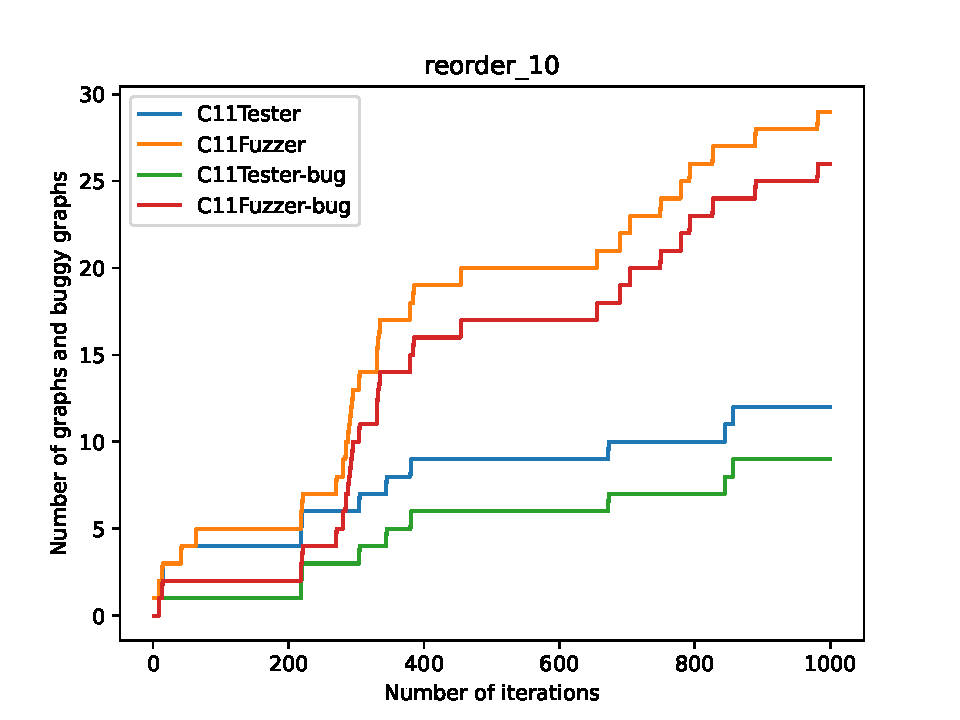
\includegraphics[width=\textwidth]{figure/hardbug/reorder_10_bug.pdf}
		\caption{reorder-10}
		\label{hard:reorder-10}
	\end{minipage}
	\hfill
	\begin{minipage}{0.45\textwidth}
		\centering
		% This empty minipage will help the last image to be aligned to the left
	\end{minipage}



\end{figure}










\subsection{\ref*{RQ:coverage}: Fuzzer vs C11Tester}

Using the 11 benchmarks, we evaluate the ability of finding unique execution graphs of both the fuzzer and C11Tester. The metric used is the number of different execution graphs discovered over $N$ iterations. Table \ref{c11fuzzer-bench1} and \ref{c11fuzzer-bench2} show the number of unique executions found by two approaches. It can be seen that the fuzzer is able to find a larger number of different execution graphs in a fixed number of iterations than C11Tester with the random-based searching strategy in most of the benchmarks, with the average improvement of 27.0\%. The improvements are calculated by:
\[
	R_{improvement} = \frac{N_{c11Fuzzer} - N_{c11Tester} }{N_{c11Tester} } \times 100 \% ,
\]
where $N_{c11Fuzzer}$ and $N_{c11Tester}$ are the number of unique execution graphs found by C11Tester and C11Fuzzer, respectively.

\begin{table}[h!]
	\begin{tabular}{ |c|ccccc| }
		\hline
		Benchmarks  & barrier & chase-lev-deque & mpmc-queue & linuxrwlocks & mcs-lock \\
		\hline
		C11Tester   & 6969    & 6244            & 4185       & 981          & 9703     \\
		C11Fuzzer   & 7741    & 8505            & 6373       & 1225         & 9994     \\
		\hline
		Improvement & 11.1\%  & 36.2\%          & 52.3\%     & 24.9\%       & 3.0\%    \\
		\hline
	\end{tabular}
	\caption{benchmarks (1)}
	\label{c11fuzzer-bench1}

\end{table}

\begin{table}[h!]
	\begin{tabular}{ |c|cccccc| }
		\hline
		Benchmarks  & dekker & rwlock-test & seqlock-test & bipartite-buf & left-right & ring-buf \\
		\hline
		C11Tester   & 395    & 9998        & 6137         & 297           & 5378       & 328      \\
		C11Fuzzer   & 494    & 9997        & 7962         & 340           & 6678       & 576      \\
		\hline
		Improvement & 25.1\% & -0.0\%      & 29.7\%       & 14.5\%        & 24.2\%     & 75.6\%   \\
		\hline
	\end{tabular}
	\caption{benchmarks (2)}
	\label{c11fuzzer-bench2}
\end{table}


In addition, Figure \ref{cover-plot1-barrier} to \ref{cover-plot1-ring-buf} draws the coverage plots for each benchmark, with orange lines representing the fuzzer and blue lines representing the random tester. It can be obeserved that in all of these cases the fuzzer is able to find more unique executions. In addition, in some benchmarks, see Figure \ref{cover-plot1-chase-lev-deque} or \ref{cover-plot1-mpmc-queue} for example, the fuzzer's speed of finding executions (the slop of coverage plost) is not significantly slowing down as the number of found executions grows. Some coverage plots of the fuzzer, such as in Figure \ref{cover-plot1-bipartite-buf} and \ref{cover-plot1-ring-buf}, also have some "bumps" which the random tester do not have. Such bumps are caused by some prefixes that guides to a group of new interesting executions.

\begin{figure}[H]

	\centering
	\begin{minipage}{0.45\textwidth}
		\centering
		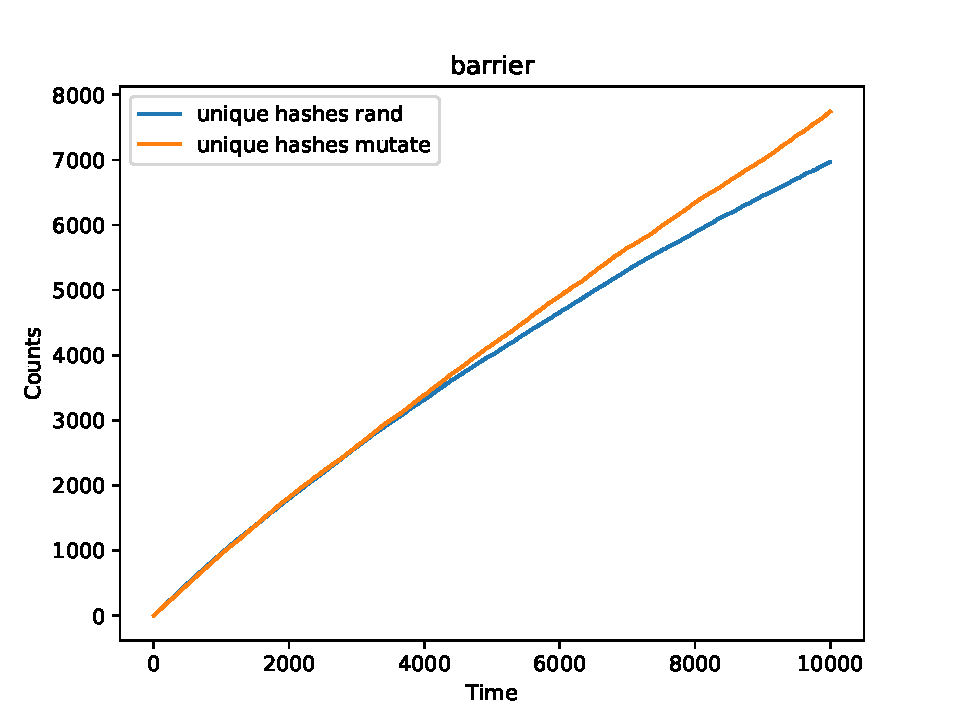
\includegraphics[width=\textwidth]{figure/barrier.pdf}
		\caption{barrier}
		\label{cover-plot1-barrier}
	\end{minipage}
	\hfill
	\begin{minipage}{0.45\textwidth}
		\centering
		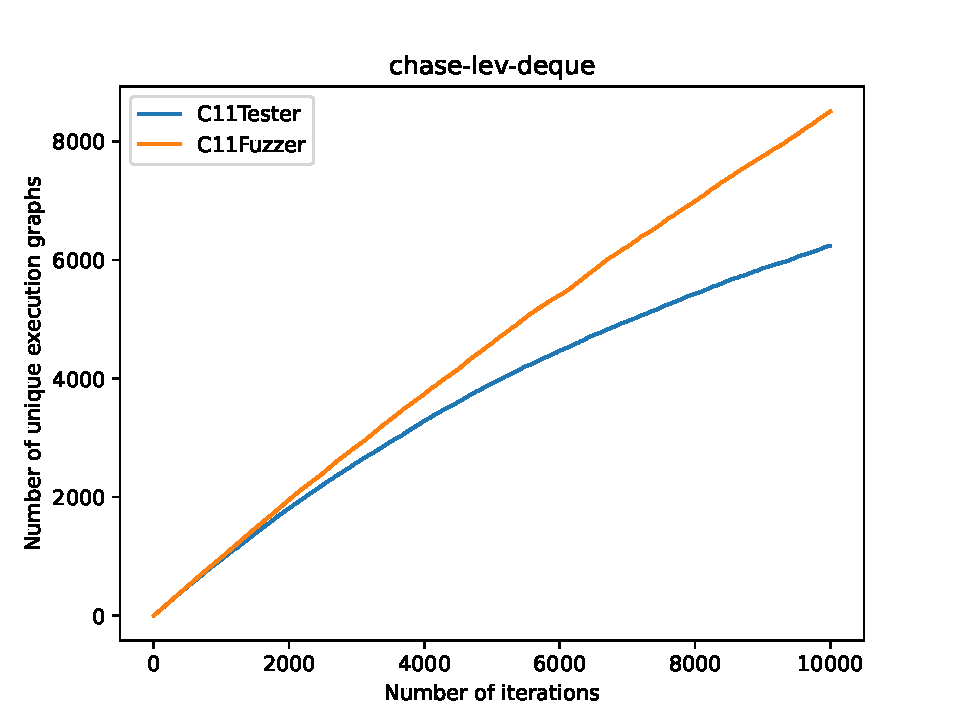
\includegraphics[width=\textwidth]{figure/chase-lev-deque.pdf}
		\caption{chase-lev-deque}
		\label{cover-plot1-chase-lev-deque}
	\end{minipage}

	\vspace{0.5cm}

	\begin{minipage}{0.45\textwidth}
		\centering
		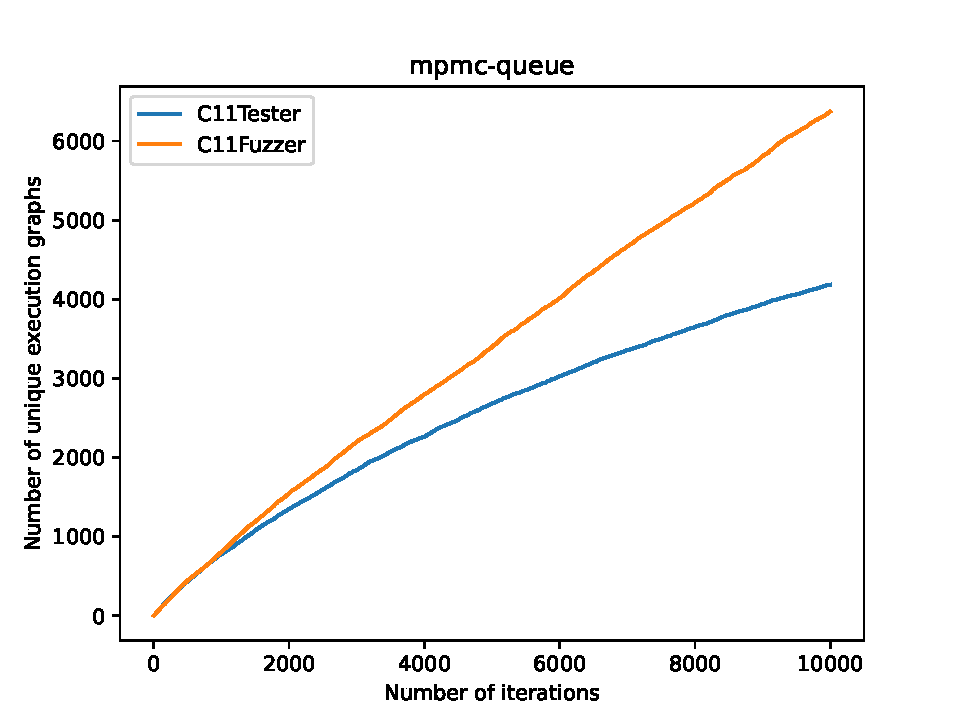
\includegraphics[width=\textwidth]{figure/mpmc-queue.pdf}
		\caption{mpmc-queue}
		\label{cover-plot1-mpmc-queue}
	\end{minipage}
	\hfill
	\begin{minipage}{0.45\textwidth}
		\centering
		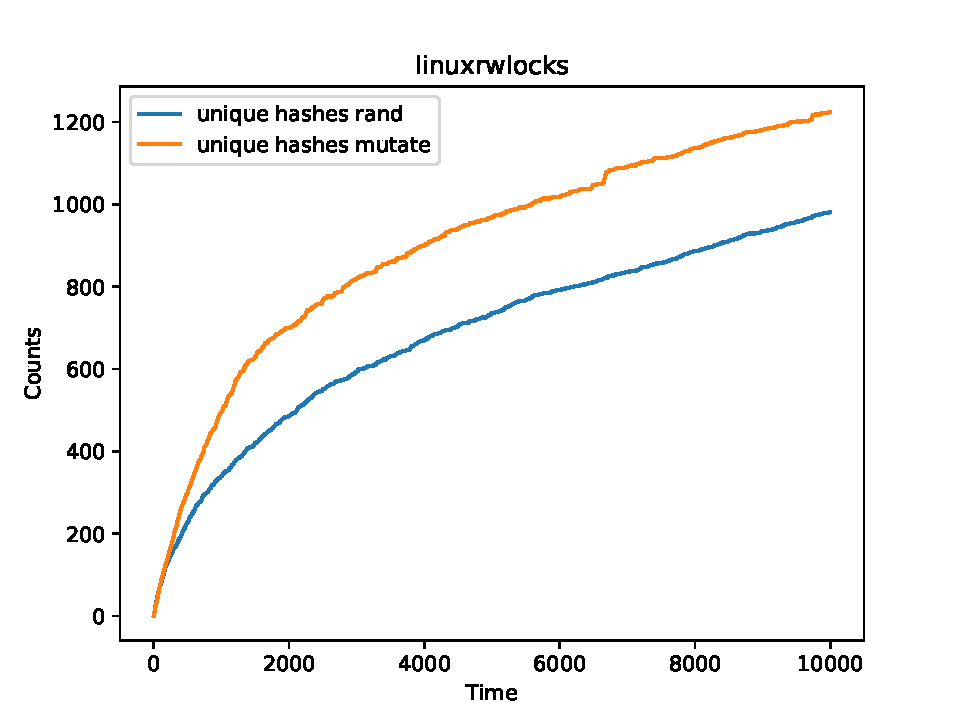
\includegraphics[width=\textwidth]{figure/linuxrwlocks.pdf}
		\caption{linuxrwlocks}
		\label{cover-plot1-linuxrwlocks}
	\end{minipage}

	\vspace{0.5cm}

	\begin{minipage}{0.45\textwidth}
		\centering
		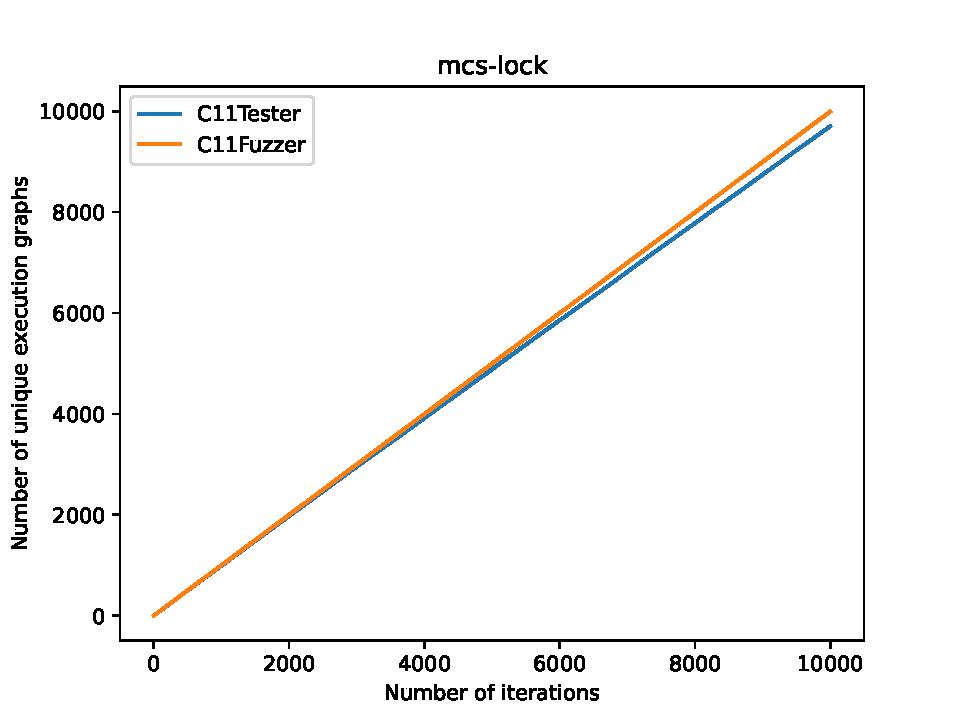
\includegraphics[width=\textwidth]{figure/mcs-lock.pdf}
		\caption{mcs-lock}
		\label{cover-plot1-mcs-lock}
	\end{minipage}
	\hfill
	\begin{minipage}{0.45\textwidth}
		\centering
		% This empty minipage will help the last image to be aligned to the left
	\end{minipage}



\end{figure}



\begin{figure}[H]
	\centering
	\begin{minipage}{0.45\textwidth}
		\centering
		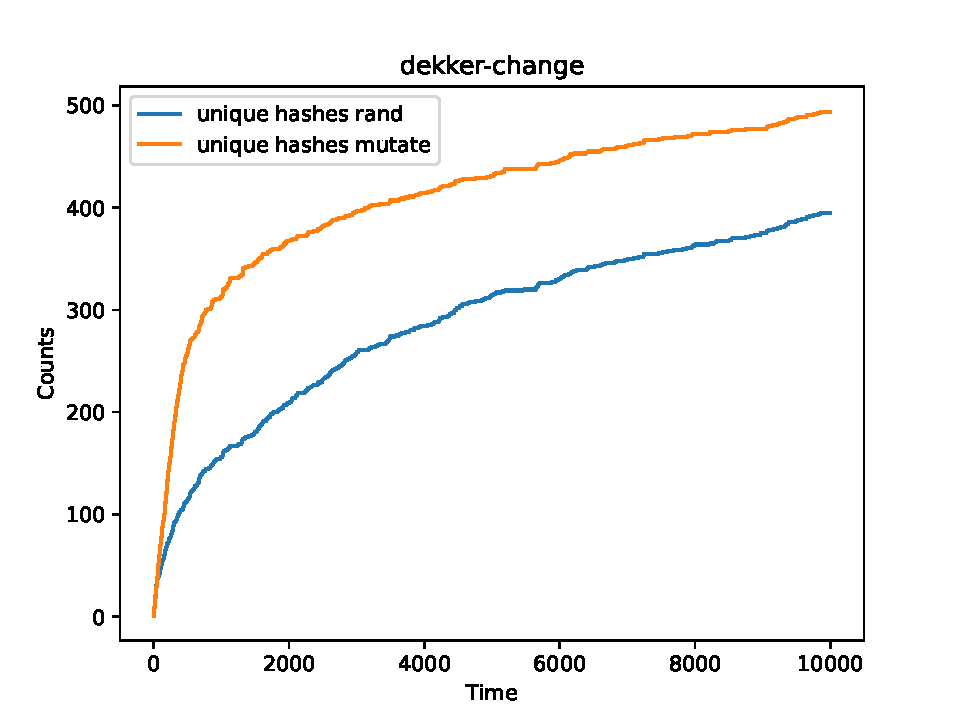
\includegraphics[width=\textwidth]{figure/dekker-change.pdf}
		\caption{dekker-change}
		\label{cover-plot1-dekker-change}
	\end{minipage}
	\hfill
	\begin{minipage}{0.45\textwidth}
		\centering
		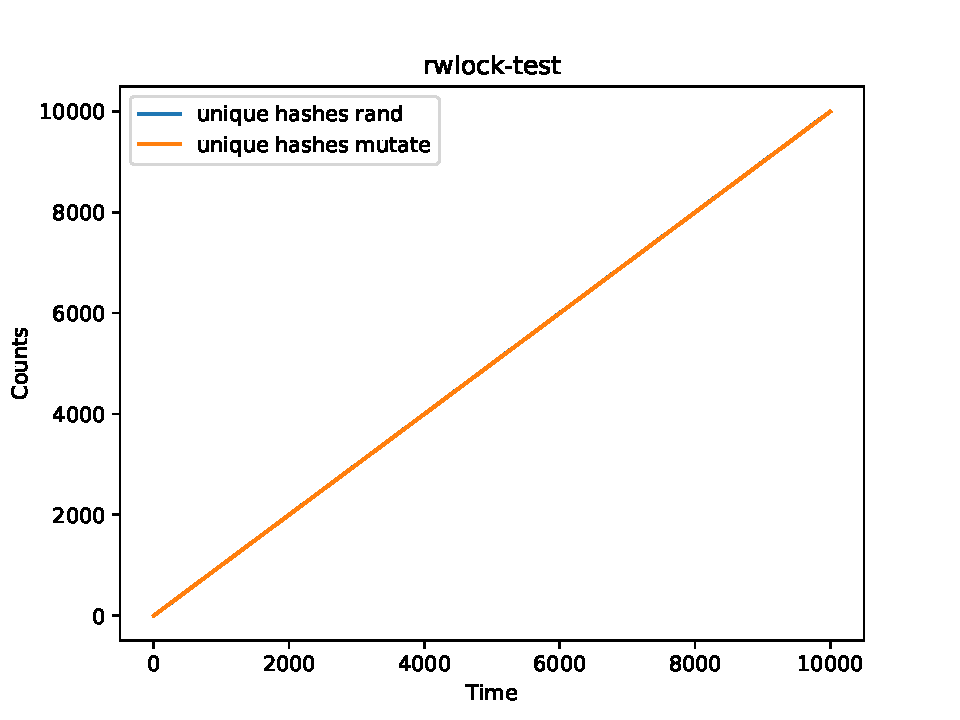
\includegraphics[width=\textwidth]{figure/rwlock-test.pdf}
		\caption{rwlock-test}
		\label{cover-plot1-rwlock-test}
	\end{minipage}

	\vspace{0.5cm}

	\begin{minipage}{0.45\textwidth}
		\centering
		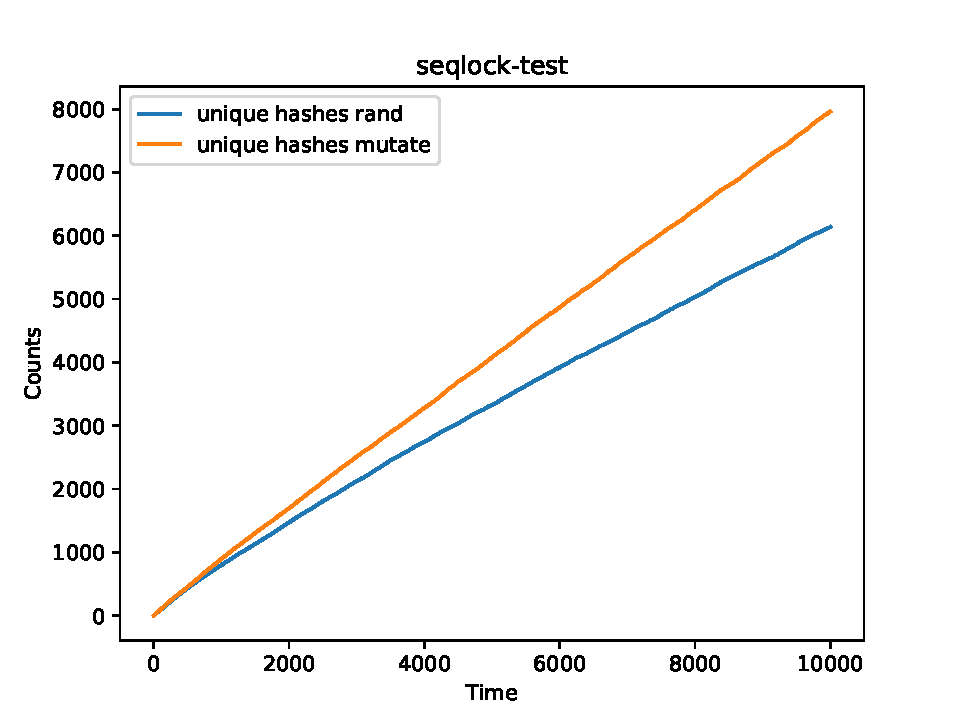
\includegraphics[width=\textwidth]{figure/seqlock-test.pdf}
		\caption{seqlock-test}
		\label{cover-plot1-seqlock-test}
	\end{minipage}
	\hfill
	\begin{minipage}{0.45\textwidth}
		\centering
		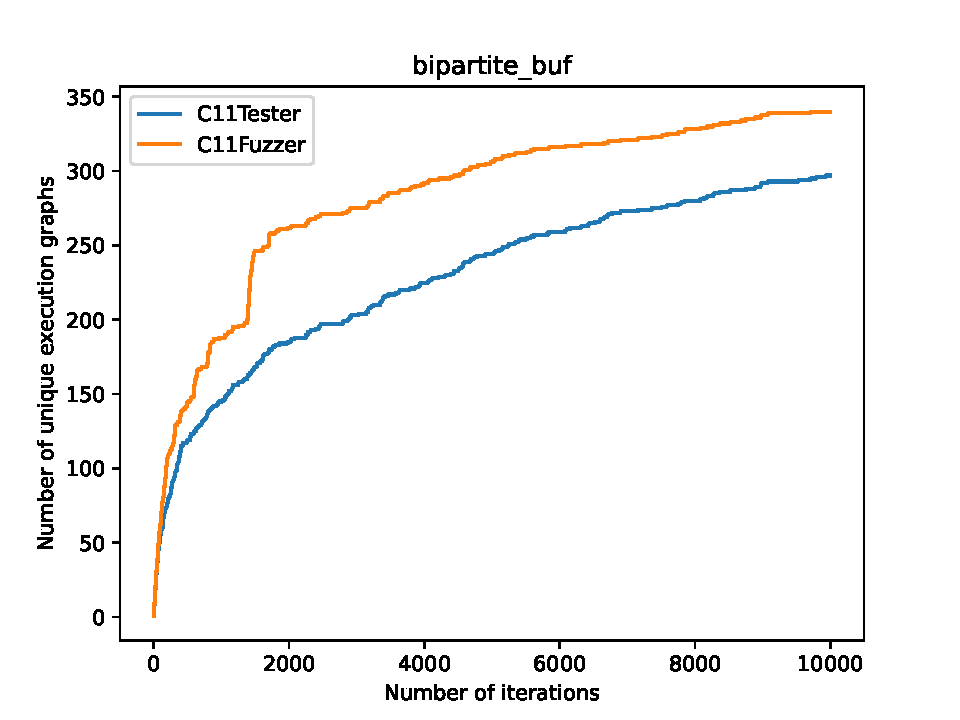
\includegraphics[width=\textwidth]{figure/bipartite_buf.pdf}
		\caption{bipartite-buf}
		\label{cover-plot1-bipartite-buf}
	\end{minipage}

	\vspace{0.5cm}

	\begin{minipage}{0.45\textwidth}
		\centering
		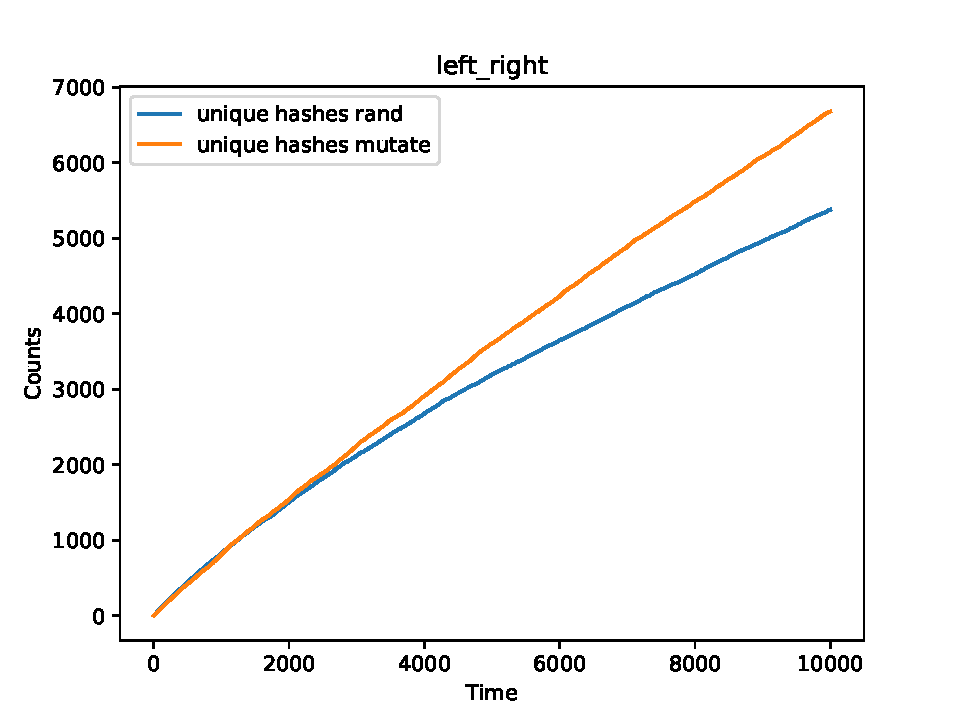
\includegraphics[width=\textwidth]{figure/left_right.pdf}
		\caption{left-right}
		\label{cover-plot1-left-right}
	\end{minipage}
	\hfill
	\begin{minipage}{0.45\textwidth}
		\centering
		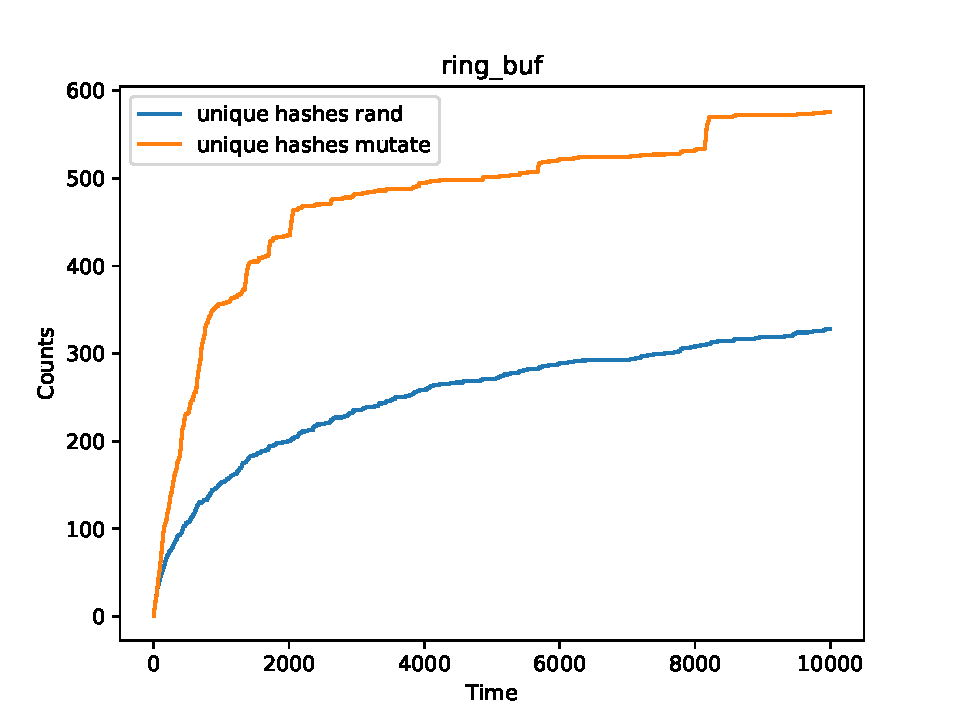
\includegraphics[width=\textwidth]{figure/ring_buf.pdf}
		\caption{ring-buf}
		\label{cover-plot1-ring-buf}
	\end{minipage}

\end{figure}

\subsection{\ref*{RQ:coverage}: C11Fuzzer vs PCTWM}

PCTWM \cite{pctwm} is a state-of-art weak concurrency tester that expands the idea of PCT, which constrains the cope of exploring executions. It is expected that PCTWM should cover a smaller range of execution graphs than that of C11Tester, which performs an unbounded random search. A subset of the benchmarks described above a tested with the same configurations of bug depth and communication events, shown in Table \ref{pctwm-configs}.

\begin{table}[h]
	\begin{tabular}{ |c|ccc| }
		\hline
		Benchmark       & bug depth (d) & communication (k) & history (h) \\
		\hline
		barrier         & 1             & 10                & 2           \\
		chase-lev-deque & 2             & 56                & 1           \\
		mcs-lock        & 1             & 16                & 1           \\
		seqlock-test    & 4             & 18                & 1           \\
		linuxrwlocks    & 5             & 100               & 10          \\
		mpmc-queue      & 2             & 17                & 2           \\
		\hline
	\end{tabular}
	\caption{PCTWM parameters}
	\label{pctwm-configs}
\end{table}

Figure \ref{pctwm-barrier} to \ref{pctwm-mpmc-queue} show the coverage plots of number of unique executions found by PCTWM, C11Fuzzer and C11Tester. It can be obeserved that PCTWM's bounded searching scope is usually lower than C11Tester's unbounded random searching scope, which is lower than C11Fuzzer's.

\begin{figure}[H]
	\centering

	\begin{minipage}{0.45\textwidth}
		\centering
		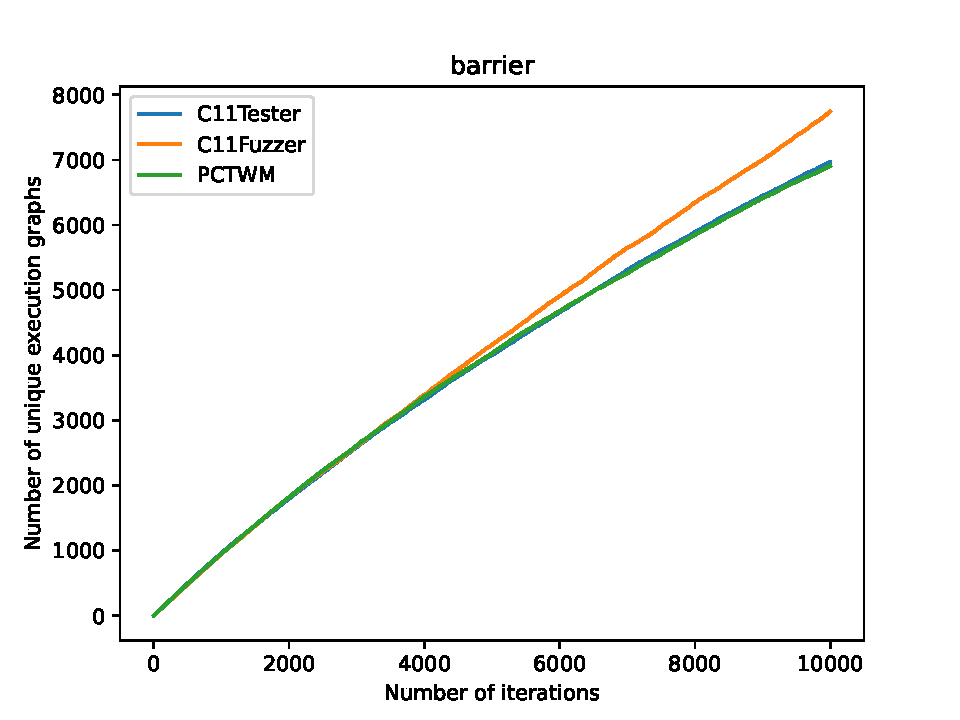
\includegraphics[width=\textwidth]{figure/pctwm/barrier.pdf}
		\caption{barrier}
		\label{pctwm-barrier}
	\end{minipage}
	\hfill
	\begin{minipage}{0.45\textwidth}
		\centering
		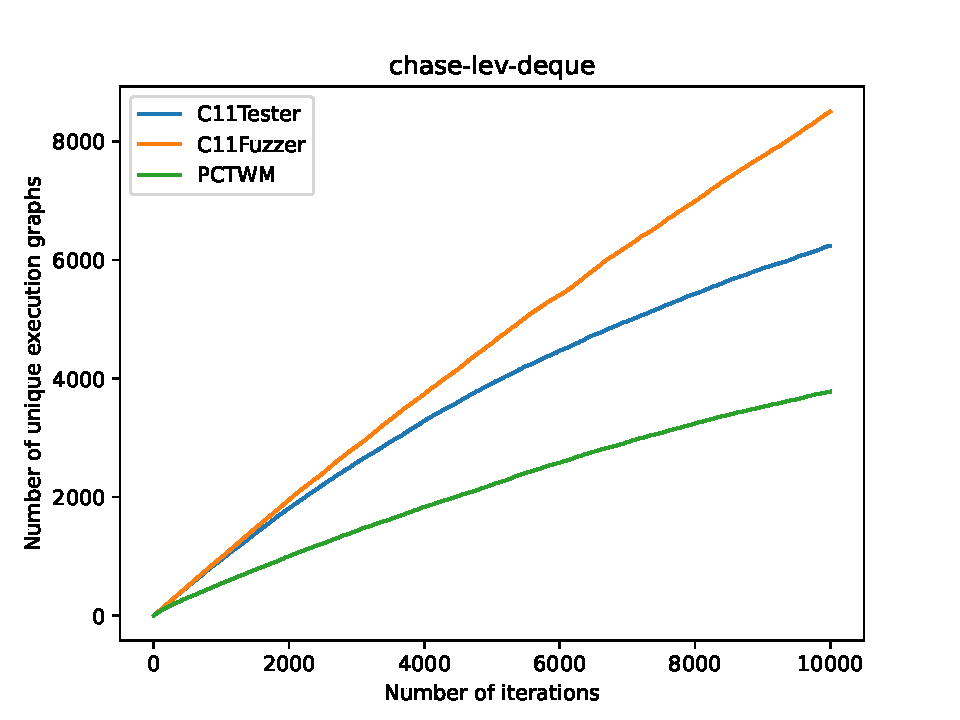
\includegraphics[width=\textwidth]{figure/pctwm/chase-lev-deque.pdf}
		\caption{chase-lev-deque}
		\label{pctwm-chase-lev-deque}
	\end{minipage}
	\vspace{0.5cm}

	\begin{minipage}{0.45\textwidth}
		\centering
		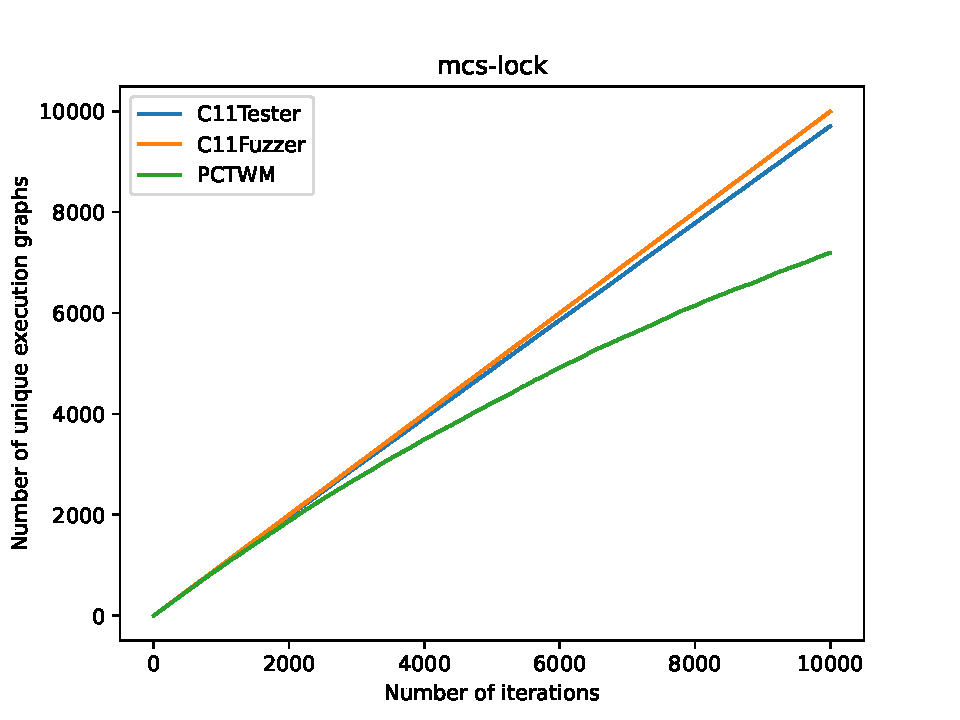
\includegraphics[width=\textwidth]{figure/pctwm/mcs-lock.pdf}
		\caption{mcs-lock}
		\label{pctwm-mcs-lock}
	\end{minipage}
	\hfill
	\begin{minipage}{0.45\textwidth}
		\centering
		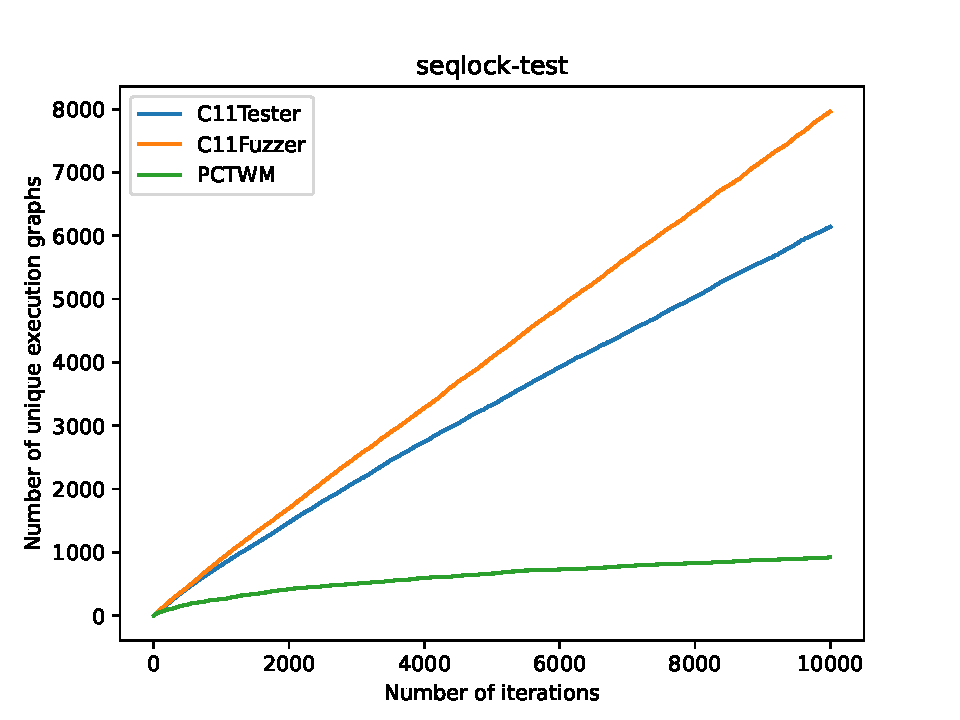
\includegraphics[width=\textwidth]{figure/pctwm/seqlock-test.pdf}
		\caption{seqlock-test}
		\label{pctwm-seqlock-test}
	\end{minipage}
	\vspace{0.5cm}

	\begin{minipage}{0.45\textwidth}
		\centering
		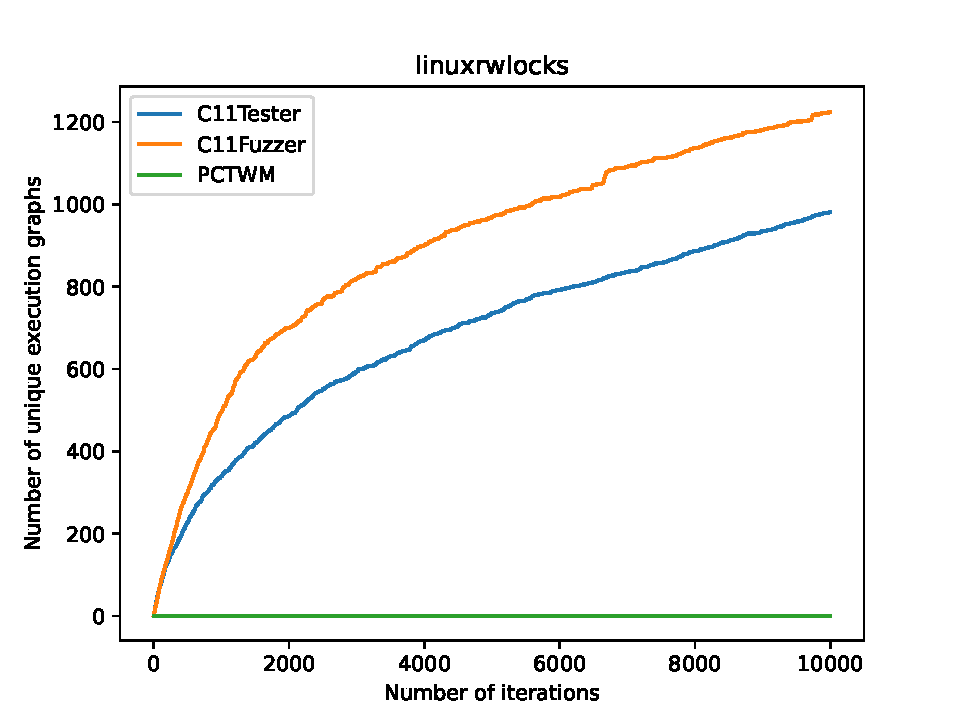
\includegraphics[width=\textwidth]{figure/pctwm/linuxrwlocks.pdf}
		\caption{linuxrwlocks}
		\label{pctwm-linuxrwlocks}
	\end{minipage}
	\hfill
	\begin{minipage}{0.45\textwidth}
		\centering
		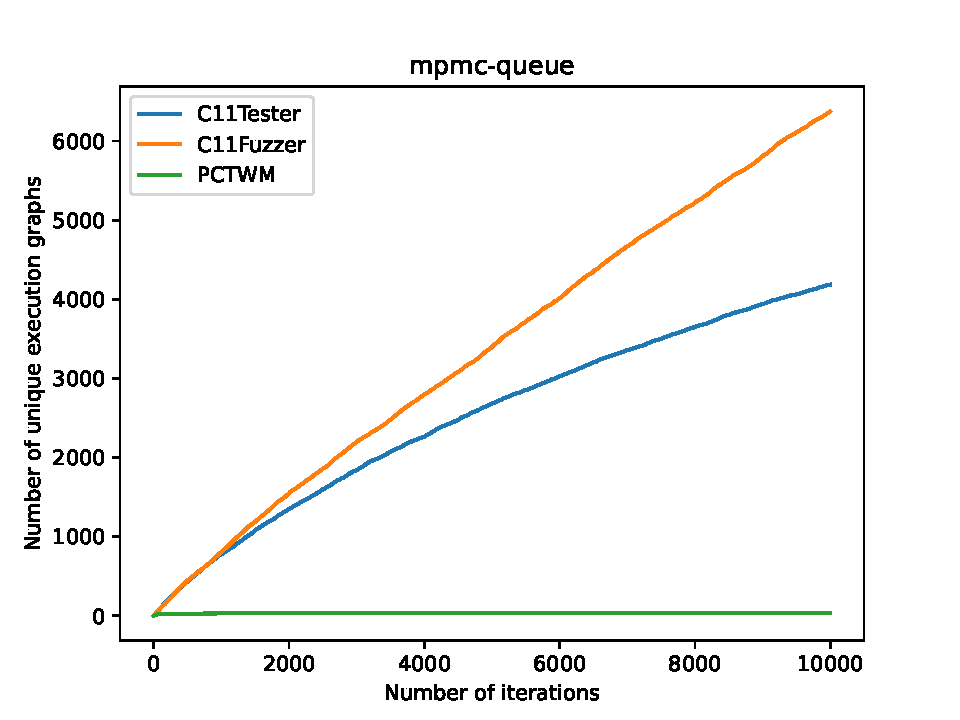
\includegraphics[width=\textwidth]{figure/pctwm/mpmc-queue.pdf}
		\caption{mpmc-queue}
		\label{pctwm-mpmc-queue}
	\end{minipage}
	\vspace{0.5cm}

\end{figure}


\subsection{\ref*{RQ:bug}: Bug hitting rate}

The design of the fuzzer is not biased on finding bugs, but it is also interested whether covering a wider range of execution graphs will improve the bug hitting rate. Some of the above benchmarks contains injected bugs, i.e. inappropriate using of synchronization primitives, which can introduce either data races or assertion failures. The bug hitting rate is computed by:
\[
	R_{bug} = \frac{N_{bug}}{N},
\]
where $N_{bug}$ is the number of different buggy executions found over $N$ iterations. Since all benchmarks are executed $N$ times, higher number of bugs represent higher bug hitting rate. Table \ref{buggy1} and \ref{buggy2} show the results from the benchmarks.


\begin{table}[h!]
	\begin{tabular}{ |c|ccccc| }
		\hline
		Benchmarks & barrier & chase-lev-deque & mpmc-queue & linuxrwlocks & mcs-lock \\
		\hline
		C11Tester  & 5789    & 5895            & 2341       & 976          & 8525     \\
		C11Fuzzer  & 6993    & 5858            & 5858       & 1220         & 9418     \\
		\hline
	\end{tabular}
	\caption{bug hitting rate (1)}
	\label{buggy1}

\end{table}

\begin{table}[h!]
	\begin{tabular}{ |c|cccccc| }
		\hline
		Benchmarks & dekker & rwlock-test & seqlock-test & bipartite-buf & left-right & ring-buf \\
		\hline
		C11Tester  & 5      & 4697        & 3872         & 297           & 1478       & 328      \\
		C11Fuzzer  & 5      & 4736        & 5009         & 340           & 1488       & 576      \\
		\hline
	\end{tabular}
	\caption{bug hitting rate (2)}
	\label{buggy2}
\end{table}

It can be obeserved that except for dekker benchmark, which in total has 5 different bugs, C11Fuzzer is able to find more bugs in other benchmarks.



\subsection{\ref*{RQ:overhead}: Real-world applications}

The fuzzer is composed of a python script that performs mutation and file IO's and a compiled binary that is hooked to the executed program. For overhead evaluation, several things are measured:
\begin{itemize}
	\item The scripting overhead of the random version and the fuzzing version. Substracting them yields the overhead of mutation and IO's.
	\item The time used by the binary to load the decisions for replay.
	\item The time used for the binary to execute.
\end{itemize}

We test our fuzzer using a real-world application, iris, which is an asynchronous logging library that makes extensive use of atomic operations. Both C11Tester and C11Fuzzer are tested $N=100$ times and an average of the overhead per execution is taken. Table \ref{overhead} shows the measurement results. It can be seen that the mutation takes up most of the overhead. A future improvement could be writing the fuzzer in a compiled language and transfer the heavy file IO into memory.

\begin{table}[h!]
	\centering
	\begin{tabular}{ |c|cccc| }
		\hline
		Items     & script & binary & mutation & load-replay \\
		\hline
		C11Tester & 1.50s  & 39.51s & 0s       & 0s          \\
		C11Fuzzer & 8.9s   & 40.5s  & 7.4s     & 2.9s        \\
		\hline
	\end{tabular}
	\caption{overhead (per execution)}
	\label{overhead}
\end{table}

\burcu{TODO: Discuss the results/plots. What do we observe? What can we say about the results?}

 
\chapter{\label{cha:genmc}Fuzzing with GenMC}

In this chapter we first present an overview of GenMC. Then we present three different mutation strategies and show their effectiveness in the end.

\section{Overview of GenMC}

GenMC is an model checker for C programs, supporting a variaty of memory models, including RC11\cite{RC11}, IMM\cite{IMM} and LKMM\cite{LKMM} memory models. It uses Kater\cite{Kater} to automatically generate axiomatic memory models that provides the specified interfaces. The memory models to be checked can be selected by the user via command line arguments, with RC11 being the default model. It incorporates an LLVM-based interpreter that compiles the target program into LLVM-IR (intermediate representation) and generates execution graphs in accordance with the specified memory model. Data races, assertion failures and other errors will be reported when detected. GenMC has two modes: estimation mode and verification mode. In estimation mode, the GenMC driver randomly collects a sample of execution graphs, independantly, to get an estimation of the size of the state space and time to finish verification. After estimation, the driver performs an exhaustive enumeration of execution graphs in the verification mode and halts when errors are encountered. The estimation mode can be disabled by command line options, too.

Both the estimation and verification modes share the same set of interfaces, with some functionality turned off during estimation. Since the fuzzer aims to improve randomized testing, here we mainly describes GenMC's estimation mode and show its customization points for our fuzzer.

The core component of GenMC is its driver, an instance created according to command line options including the chosen memory model, transformation options, exploration strategies, etc. The driver is responsible for calling the interpreter to transform the target program into LLVM-IR, constructing execution graphs, checking consistency, and reporting errors. The interpreter is derived from LLVM's execution engine and instruction visitor, used to interpret the source code and keep relevant execution information. The interpreter will ask the scheduler of the driver to fetch the next instruction. Normally, the scheduler randomly picks the next thread and fetches the next instruction of that thread, with some special cases such as RMW instructions, prioritized threads, or reads that need to be rescheduled. Then the interpreter handles each instruction following the visitor pattern. Some special instruction-handling functions are overridden by the driver, such as handleLoad, handleStore, handleFence, and handleSpinStart. For instance, the handleLoad function will pick a write value allowed by the memory model for the load instruction and add it to the execution graph, and the handleStore function will add it to the execution graph and insert it into the modification order (coherence) at some proper place, as well as checking consistency and reporting possible data races.

The execution graph is composed of events, each having a label indicating its position in the graph and other information about the event itself. It also maintains a map that records the store events of each memory location. An event can be looked up using its position, which is a pair of thread id and its index in that thread. Additional information is also stored in the label. For example, a read event label also contains its reads-from information and atomic ordering. Both the stamp and the position uniquely identify an event in a single graph; however, the stamp is determined by the order of adding events to the graph and hence will vary across explorations, while the position is determined by the source code of the tested program.

The driver has a stack of executions, called execStack. Each execution has an execution graph instance and a workqueue. The workqueue stores the exploration operations, called Revisit, to be conducted, on the corresponding graph. The driver fetches an item each time from the workqueue and "revisit" it. When the workqueue is empty, the driver is informed that no more actions are needed for the current graph, so it pops out the current execution from the execStack and continues with other executions. When the execStack is empty the driver finishes its job and report the statistics. In estimation mode, only one kind of Revisit, RerunForwardRevisit, is used, which indicates the driver to reset the execution graph to its initial state and start over the next iteration.

The above mentioned exploration procedure is listed in Algorithm. \ref{driver::run}.

\begin{algorithm}
	\caption{GenMC driver explore}
	\label{driver::run}
	\begin{algorithmic}[1]
		\STATE $EE \leftarrow \text{getInterpreter}()$
		\STATE $execStack \leftarrow []$

		\WHILE{not \text{isHalting}()}
		\STATE /* Continue with the current graph */
		\STATE $EE$.run()
		\STATE $r \leftarrow RerunForwardRevisit$
		\STATE $stamp \leftarrow 0$
		\STATE pushRevisit($execStack$[last], $r$, $stamp$)

		\STATE $validExecution \leftarrow \text{false}$
		\WHILE{not $validExecution$}
		\STATE $[{stamp}, {item}] \leftarrow \text{getNextItem}(execStack[last].workqueue)$
		\IF{$item$ is empty}
		\STATE execStack.pop()
		\IF{not execStack.empty()}
		\STATE \text{continue}
		\ELSE
		\RETURN
		\ENDIF

		\ELSE
		\STATE $g \leftarrow execStack[\text{last}].graph$
		\STATE cutToStamp($g$, $stamp$)
		% \STATE 
		\STATE $validExecution \leftarrow \text{isConsistent}(g)$   /*always true for graphs cut from RerunForwardRevisit*/
		\ENDIF
		\ENDWHILE
		\ENDWHILE
	\end{algorithmic}
\end{algorithm}





\section{Customazation points of GenMC}

In the estimation mode, the driver pushes a RerunForwardRevisit and a zero stamp to the workqueue at the end of each execution, so the graph will always be reset to an empty state, which stays at the end of execStack. It is also viable to push other Revisit objects to the workqueue and the driver will cut the graph accordingly. In addition, we could also cut the graph manually and push it together with a latest stamp so the driver will not cut it again. If the manually cut graph is consistent, the interpreter will continue and finish exploration with it. Both pushing other Revisit and manually cutting the graph serve as the mutation part of our fuzzer. The driver has a function, getRfsApproximation, that can provide a list of stores that a read can read from, so the fuzzer can pick a different store from that list.

\section{Fuzzer implementation}

Similar to what is discussed in section~\ref{c11fuzzer:implementation}, several functions need to be implemented.

\begin{itemize}
	\item A hash function that computes a unique identifier for an execution graph.
	\item A function that mutate the previous execution graph and produces a prefix of the mutated graph.
\end{itemize}


\subsection{hash function for execution graphs}
Firstly the hash function for a single event should be defined, as shown in Algorithm~\ref{alg:hash-eventlabel}

\begin{algorithm}
	\caption{Hashing an EventLabel}
	\label{alg:hash-eventlabel}
	\begin{algorithmic}[1]
		\STATE \textbf{Input:} EventLabel $lab$
		\STATE \textbf{Output:} Hash value $h$ = hash($lab$)
		\STATE $h \leftarrow 0$
		\STATE $pos \leftarrow lab.\text{getPos}()$
		\STATE \text{hash\_combine}(h, pos.thread)
		\STATE \text{hash\_combine}(h, pos.index)

		\IF{$lab$ is a ReadLabel}
		\IF{$lab$.getRf() is not empty}
		\STATE $slab \leftarrow$ $lab$.getRf()
		\STATE \text{hash\_combine}($h$, hash($slab$))
		\ENDIF
		\ENDIF
		\RETURN $h$
	\end{algorithmic}
\end{algorithm}

Then the events are iterated by thread id and indices to compute the hash value of the graph, as listed in Algorithm~\ref{alg:hash-executiongraph}.


\begin{algorithm}
	\caption{Hashing an ExecutionGraph}
	\label{alg:hash-executiongraph}
	\begin{algorithmic}[1]
		\STATE \textbf{Input:} ExecutionGraph $g$
		\STATE \textbf{Output:} Hash value $h$ = hash($g$)
		\STATE $h \leftarrow 0$
		\FOR{$i \leftarrow 0$ to $g.getNumThreads() - 1$}
		\FOR{$j \leftarrow 0$ to $g.getThreadSize(i) - 1$}
		\STATE $lab \leftarrow g.getEventLabel(\text{Event}(i, j))$
		\STATE \text{hash\_combine}(h, \text{hash}($lab$))
		\ENDFOR
		\ENDFOR
		\RETURN $h$
	\end{algorithmic}
\end{algorithm}

\subsection{mutation methods}

The mutation process is composed of two steps: changing an rf relation and cutting the graph. The driver has provided a function, getRfsApproximation, that calculates a list of possible stores given a read event. It first collects a list of coherent stores restricted by the memory model. In RC11, it selects all concurrent stores and the latest store in mo before the provided read. The fuzzer first picks out all read events that have multiple store choices and pairs each read with each of its alternative stores. Then the fuzzer randomly selects one of these pairs for mutation. Here we denote the selected read event as $R$, its original store as $S_{old}$, and the newly selected store as $S$. In accordance to GenMC's terminology, the word "view" is used to represent a subset of events in an execution graph. Here a "cut view" represents the view of the current graph to be kept in the following cutting strategies, which serves as a prefix defined in Algorithm~\ref{fuzzer}. The fuzzer implements three different cutting strategies, described as follows:

\paragraph{Revisit cut} It constructs the ReadForwardRevisit and BackwardRevisit objects and pushes them to the workqueue directly. These two kinds of Revisit's are defined in GenMC, used in its verification mode. We first compare the timestamps of $R$ and $S$. If $R$ has a greater stamp, a ReadForwardRevisit will be constructed. When the driver retrieves a ReadForwardRevisit from the workqueue, it removes all events whose stamps are greater than $R$. Since $S$'s stamp is smaller, it will be kept. Additionally, the read becomes the latest event added to the graph, hence the events that may no longer be valid due to the change in $R$'s rf will not be retained. This cut view can be denoted as $preds_{R}$. On the other hand, if $S$ has a greater stamp, a BackwardRevisit will be constructed. The driver first collects all events that has smaller stamps than $R$, i.e. $preds_{R}$, similar as did in ReadForwardRevisit. Since $S$ has a greater stamp this time, it will not be included in $preds_{R}$. Then the driver computes all events that are porf predecessors of $S$, denoted as $pporf_{S}$. The cut view is the union of the two sets of events, $preds_{R} \cup pporf_{S}$ and the rest of the graph will be cut.

\paragraph{Minimal cut} This cut strategy aims to retain as little events as possible. It only keeps those events that are both porf predecessors of $R$ and $S$. The events in unrelated threads (concurrent events) will be dropped. The minimal cut view can be written as $pporf_{R} \cup pporf_{S}$

\paragraph{Maximal cut} This cut strategy aims to retain as many events as possible. In maximal cut, the unrelated events, which are removed in minimal cut, will be kept. It only removes the events that are porf successors of the read. To get this set of events, the fuzzer iterates through all events in the graph. For each event, if the $R$ is not a porf predecessor of it, it will be added into the set. Because the maximal cut will include more events into the cut view, some special attention needs to be paid to the "pair relations". For example, if a thread-join event is to be added into the view, both itself and its corresponding thread's thread-finish event should not be porf successors of $R$. The maximal cut view can be represented by $\{e \in G \mid R \notin pporf_e, \  R \notin pporf_{e's pair}\} \cup {R}$, where $G$ is the current graph to be mutated.








\section{Evaluation and discussion}

We use the following benchmarks to evaluate the fuzzer.

\paragraph{big0} A syntactic benchmark with multiple threads reading from and writing to shared memory locations using acquire-release memory orders.

\paragraph{ring-buffer} A ring buffer implementation in FreeBSD 8.0.0. Each thread enqueues a message and dequeues one from the buffer. The program checks the correctness and integrity of the messages. The ring buffer uses an array to store data. The enqueue and dequeue operations use compare-and-swap loops to update the queue head and tail pointers.

\paragraph{fib} Two threads update a Fibonacci sequence concurrently. Each update uses the previous values of two variables.

\paragraph{mpmc-queue} A multi-producer multi-consumer bounded queue implementation. It maintains three state variables that keeps track of the number of reads and writes that have been started and finished. Each writer obtains an index in the queue's array buffer using cas loop and write to that position. The readers will increment the reading index and read the data. In the test, 2 readers and 4 writers are spawned. 

\paragraph{szymanski} A szymanski mutual exclusion algorithm implementation. Each thread has a flag to inidicate its state. Before entering critical section, each thread updates its own flag and checks the other thread's flag. SC atomic fences are used for synchronization. 


\paragraph{ttaslock} A spinlock called Test-and-Test-and-Set (TTAS) lock. The lock has an atomic state variable shared by multiple threads. Before locking it, a thread first loads the flag and wait until it is not set. Locking is implemented using a loop that exchanges the state value until the old value of it is not set. In the benchmakr, two threads are luanched to update a non-atomic shared variable and asserts they read their values in the critical section. 


\begin{figure}[H]

	\centering
	\begin{minipage}{0.45\textwidth}
		\centering
		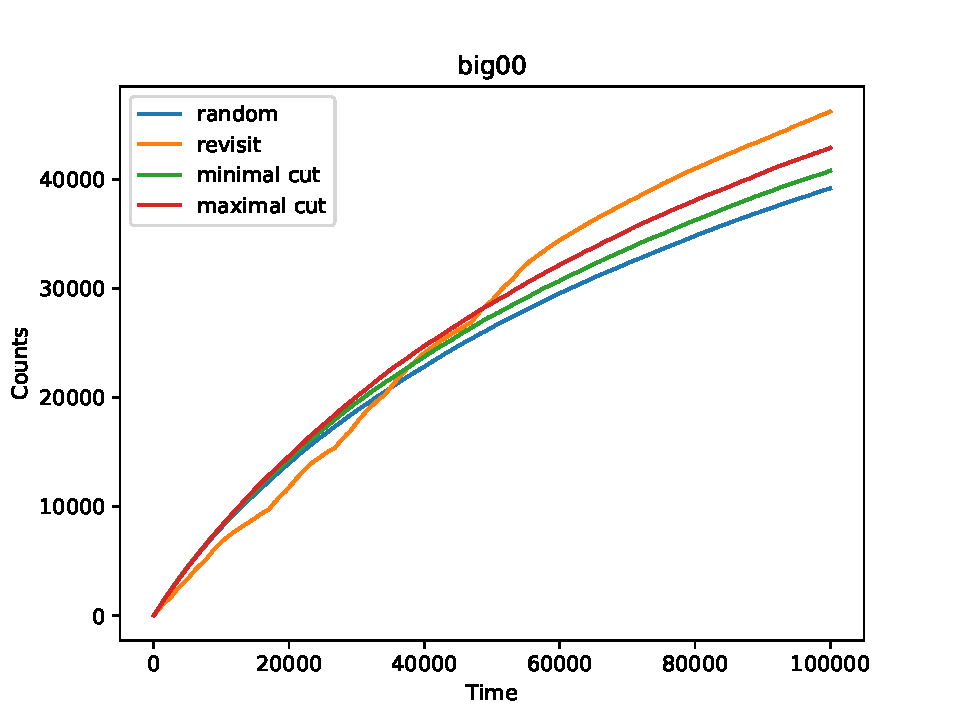
\includegraphics[width=\textwidth]{figure/genmc/big00.pdf}
		\caption{big0}
		\label{genmc:big0}
	\end{minipage}
	\hfill
	\begin{minipage}{0.45\textwidth}
		\centering
		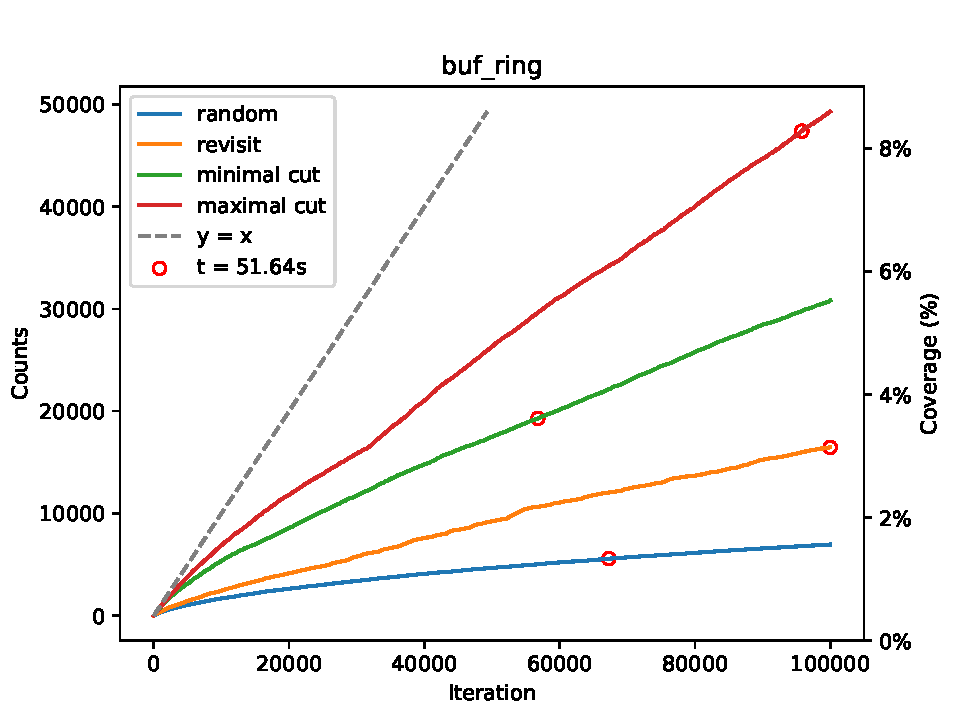
\includegraphics[width=\textwidth]{figure/genmc/buf_ring.pdf}
		\caption{ring-buffer}
		\label{genmc:buf_ring}
	\end{minipage}

	\vspace{0.5cm}

	\begin{minipage}{0.45\textwidth}
		\centering
		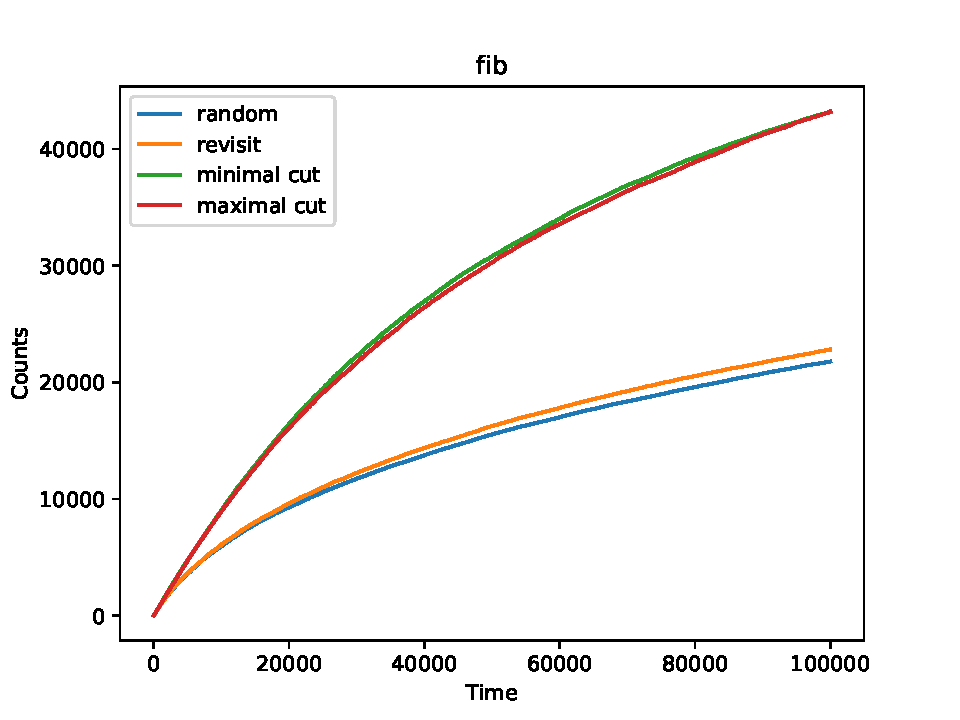
\includegraphics[width=\textwidth]{figure/genmc/fib.pdf}
		\caption{fib}
		\label{genmc:fib}
	\end{minipage}
	\hfill
	\begin{minipage}{0.45\textwidth}
		\centering
		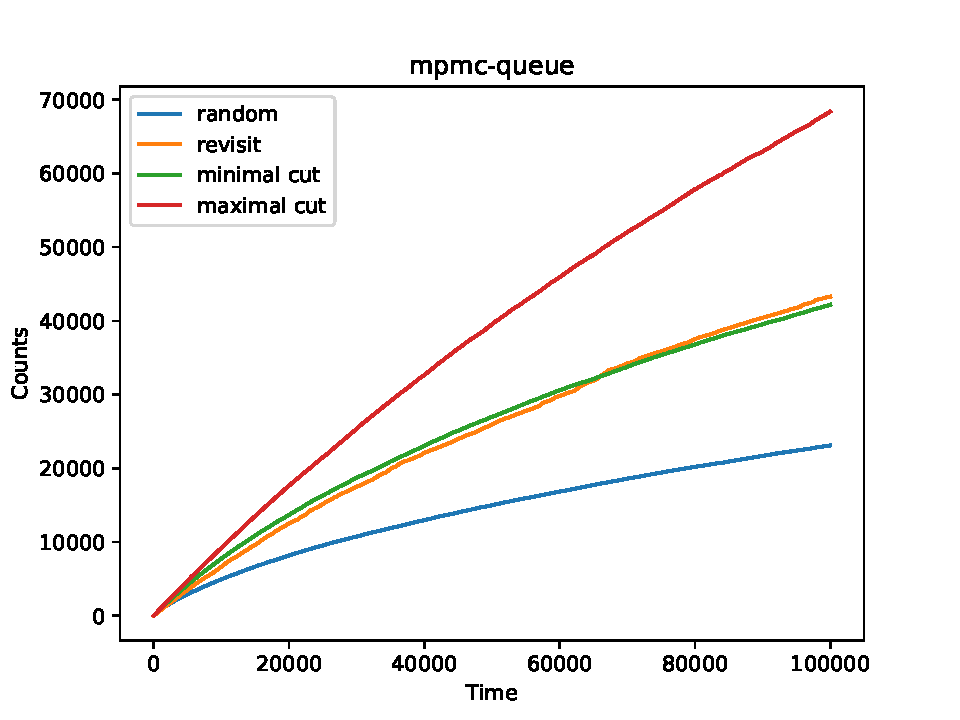
\includegraphics[width=\textwidth]{figure/genmc/mpmc-queue.pdf}
		\caption{mpmc-queue}
		\label{genmc:mpmc-queue}
	\end{minipage}

	\vspace{0.5cm}

	\begin{minipage}{0.45\textwidth}
		\centering
		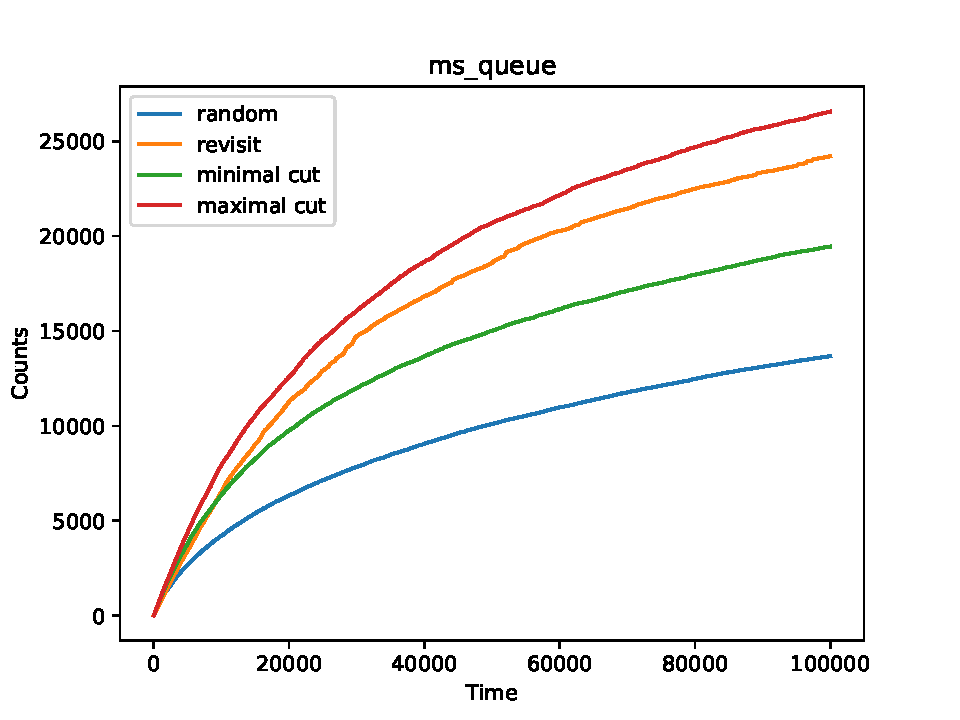
\includegraphics[width=\textwidth]{figure/genmc/ms_queue.pdf}
		\caption{ms-queue}
		\label{genmc:ms_queue}
	\end{minipage}
	\hfill
	\begin{minipage}{0.45\textwidth}
		\centering
		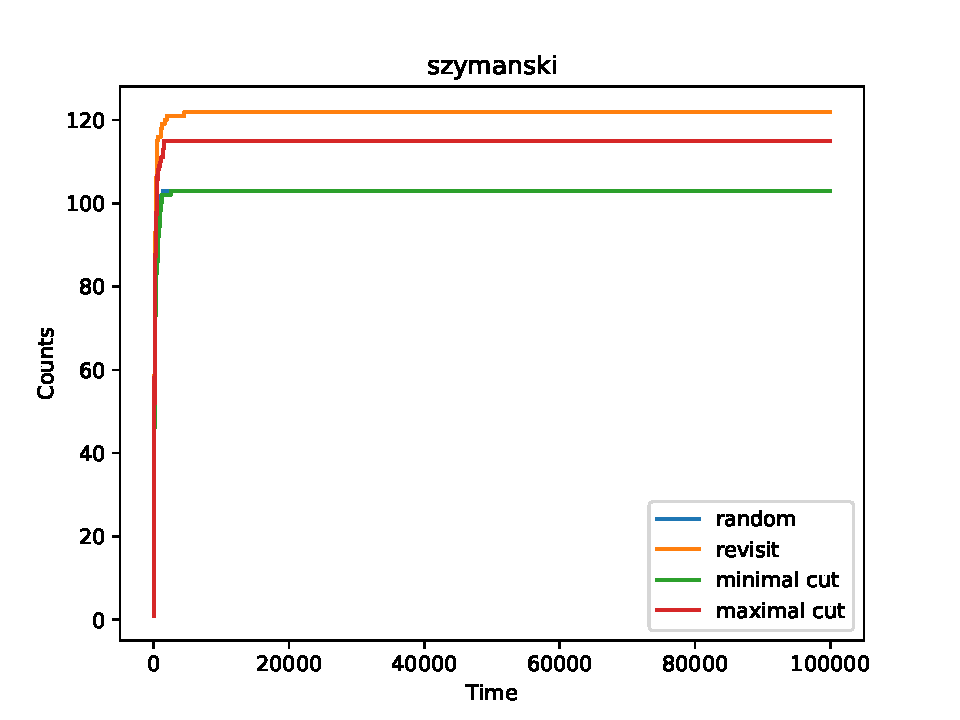
\includegraphics[width=\textwidth]{figure/genmc/szymanski.pdf}
		\caption{szymanski}
		\label{genmc:szymanski}
	\end{minipage}

	\vspace{0.5cm}
	\begin{minipage}{0.45\textwidth}
		\centering
		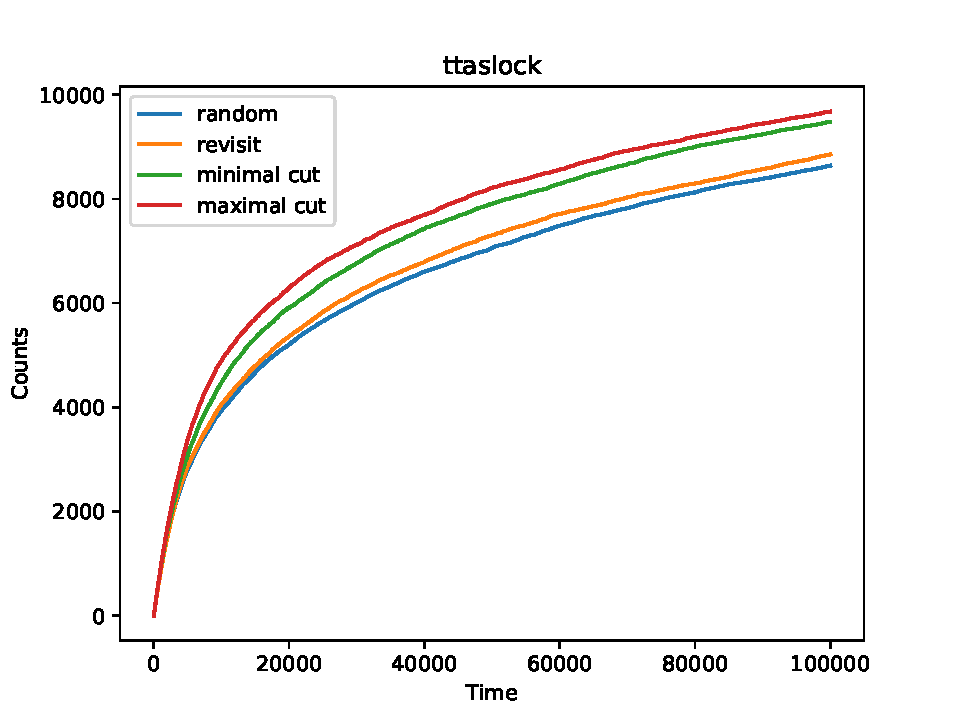
\includegraphics[width=\textwidth]{figure/genmc/ttaslock.pdf}
		\caption{ttaslock}
		\label{genmc:ttaslock}
	\end{minipage}
	\hfill
	\begin{minipage}{0.45\textwidth}
		\centering
		% This empty minipage will help the last image to be aligned to the left
	\end{minipage}



\end{figure} 
\chapter{\label{cha:related}Related Work}

Related work falls into three categories: weak memory models, model checkers and fuzzers. 

% memory model

The initial proposal for the C/C++11 memory model was made in 2008\cite{c++model-proposal}. In this proposal, the memory model is described in prose style, resulting in ambiguity and verbosity. In 2011, a formal and mathematized version was proposed, using the 




AFL\cite{afl} is a coverag guided grey-box fuzzer. The user program is intrumented with deputy functions at the entry of basicblocks evenly. The deputy functions can collect runtime information for code coverage analysis. AFL mutates the input for the program to cover new branches and execution paths. Since AFL is initially designed for sequential programs, which has deterministic results when the input and random seed are fixed, it is unaware of thread interleaving contexts. 

Muzz\cite{muzz} thread-aware grey-box fuzzing tool for multithreaded programs. Instead of instrument the user program evenly, Muzz conducts static analysis first to locate set of specific program statements on which thread-interleavings may only happen, identified as suspicious interleaving scopes. Then Muzz will instrument more deputy instructions inside these scopes. During repeated execution, the inserted functions can collect thread context information, hence the fuzzer is able to select interesting seeds that triggered unique thread interleavings. 

Conzzer\cite{conzzer} is a context-sensitive and directional concurrency fuzzing tool for data-race detection. It is motivated by the fact that some concurrent bugs only happen when two specific functions with callstacks are executed concurrently. Conzzer uses context sensitive concurrent function call pairs as the mutation target. 



CDSchecker\cite{cdschecker} is an exhaustive model checker exploring the behaviors of concurrent code under the original C/C++11 memory model based on stateless model-checking. A technique of constraint-based treatment of modification order is introduced remove redundancy from the search space. A cycle in the modification order graph corresponds to infeasibility of the constraints. CDSchecker uses depth-first search to check for cycles by adding edges to the modification order graph and rolls back when the constraints are unsatisfiable. The scalability limits and memory model support are extended by the C11Tester. 

C11Tester \cite{c11tester} is a race detector for the C/C++ memory model. It supports concurrency primitives and the weak memory behaviors allowed by the C/C++20 standard. A constraint-based algorithm is proposed to explore the modification order graph. Under the memory model constraints, decisions are made randomly when generating possible thread interleavings and atomic operation behaviors. During repeated execution, execution graphs are generated independantly without feedback information from previous iterations by default. However, C11Tester provides a plugable framework that allows for selecting the next thread and behavior from a set of legal choices.   

GenMC \cite{genmc} is a stateless model checker for C/C++ programs under weak memory models. It suports a variety of memory models such as  RC11, IMM, and LKMM, and is extendable for  further axiomatic memory models. The program is compiled into LLVM-IR for incorporating optimizations including symmetry reduction and lock-aware partial order reduction, making it possible to support different programming languages provided that its memory model is axiomatic well defined. 

% \section{Model Checkers}
 
% \lipsum{2} % add some pseudo content

% \section{Related part II}

% \lipsum{4} % add some pseudo content 
   
% \section{Related part III}

% \lipsum{1} % add some pseudo content

 

\chapter{\label{cha:conc}Conclusions and Future 
Work}

This chapter gives an overview of the project's contributions. After
this overview, we will reflect on the results and draw some
conclusions. Finally, some ideas for future work will be discussed.

\section{Contributions}

\lipsum{3} % add some pseudo content


\section{Conclusions}

\lipsum{3} % add some pseudo content

\section{Discussion/Reflection}

\lipsum{4} % add some pseudo content

\section{Future work}

\lipsum{2} % add some pseudo content

 

\bibliographystyle{plainnat}
\bibliography{thesis}

\appendix
\def\chaptername{Appendix}
\chapter{\label{cha:source-code}Source code}

% In this appendix we give an overview of frequently used terms and
% abbreviations.

In this appendix we provide the source code repositories used in this thesis and instructions on how to use them.

\section{Fuzzer implementation in C11Tester}

The source code is available at GitHub: \href{https://github.com/lililuanluan/c11tester-fuzz.git}{https://github.com/lililuanluan/c11tester-fuzz.git}.


\begin{itemize}
    \item Download and install the vagrantBox\cite{vagrantBox} and VirtualBox\cite{virtualbox}. 
	\item Download the C11Tester artifact following the instructions of the C11Tester\cite{c11tester} paper.
	\item Download the fuzzer implementation from the GitHub link: \href{https://github.com/lililuanluan/c11tester-fuzz.git}{https://github.com/lililuanluan/c11tester-fuzz.git} and place the files in the \texttt{c11tester/} folder. Go to the \texttt{c11tester/benchmarks/} folder and run the \texttt{afuzzer.py} script. 
\end{itemize}


\section{Fuzzer implementation in GenMC}

The source code is available at GitHub: \href{https://github.com/lililuanluan/genmc-fuzz.git}{https://github.com/lililuanluan/genmc-fuzz.git}.

\begin{itemize}
    \item Download and install Docker\cite{docker}. 
	\item Download the GenMC artifact from paper \cite{genmc-enhance} following the instructions in its artifact\cite{genmc-enhance-artifact}.
	\item Download the \texttt{src/} and \texttt{debug-luan} folders and place them in the \texttt{~/genmc-tool/} directory. 
    \item Go to \texttt{debug-luan/} and run the \texttt{test.sh} script. 
\end{itemize}
\chapter{Requirements and Guidelines}

This chapter details some requirements and guidelines for MSc theses
submitted to the Software Engineering Research Group.

\section{Requirements}

\subsection{Layout}

\begin{itemize}
\item Your thesis should contain the formal title pages included in
  this document (the page with the TU Delft logo and the one that
  contains the abstract, student id and thesis committee). Usually
  there is also a cover page containing the thesis title and the
  author (this document has one) but this can be omitted if desired.
 
\item Base font should be an 11 point serif font (such as Times, New
  Century Schoolbook or Computer Modern). Do not use sans-serif fonts
  such as Arial or Helvetica. \textsl{Sans-serif type is intrinsically
  less legible than seriffed type} \cite{Whe95}.

\item The final thesis and drafts submitted for reviewing should be
printed double-sided on A4 paper.
\end{itemize}

\subsection{Content}

\begin{itemize}
\item The thesis should contain the following chapters:
\begin{itemize}
\item Introduction.

  Describes project context, goals and your research question(s). In
  addition it contains an overview of how (the remainder of) your
  thesis is structured.

\item One or (usually) more ``main'' chapters.

  Present your work, the experiments conducted, tool(s) developed,
  case study performed, etc.

\item Overview of Related Work

  Discusses scientific literature related to your work and describes
  how those approaches differ from what you did.

\item Discussion/Evaluation/Reflection

  What went well, what went less well, what can be improved?

\item Conclusions, Contributions, and (Recommendations for) Future Work

\item Bibliography

\end{itemize}
\end{itemize}


\subsection{Bibliography}

\begin{itemize}
\item Make sure you've included all required data such as journal,
  conference, publisher, editor and page-numbers. When you're using
  \textsc{Bib}\TeX{}, this means that it won't complain when running
  \texttt{bibtex your-main-tex-file}.
 
\item Make sure you use proper bibliographic references. This
  especially means that you should avoid references that \textbf{only}
  point at a website and not at a printed publication.

  For example, it's OK to add a URL with the entry for an article
  describing a tool to point at its homepage, but it's not OK to just
  use the URL and not mention the article.
\end{itemize}


\section{Guidelines}

\begin{itemize}

\item The main chapters of a typical thesis contain approximately 50
  pages.

\item A typical thesis contains approximately 50 bibliographic
  references.

\item Make sure your thesis structure is balanced (check this in the
  table of contents). 

  Typically the main chapters should be of equal length. If they aren't,
  you might want to revise your structure by merging or splitting some
  chapters/sections.

  In addition, the (sub)section hierarchies with the chapters should
  typically be balanced and of similar depth. If one or more are much
  deeper nested than others in the same chapter this generally signals
  structuring problems.

\item Whenever you submit a draft of your thesis to your supervisor
  for reviewing, make sure that you have checked the spelling and
  grammar.  Moreover, \emph{read it yourself at least once from start
  to end, before submitting to your supervisor}.

  \textbf{Your supervisor is not a spelling/grammar checker!}

\item Whenever you submit a second draft, include a short text which
  describes the changes w.r.t. the previous version. 

\end{itemize}






\end{document}
